\documentclass[review]{elsarticle}

\usepackage[utf8]{inputenc}
\usepackage{graphicx}
\usepackage{amsmath}
\usepackage{stfloats}
\usepackage{afterpage}
\usepackage{amssymb}
\usepackage{color}
\usepackage{verbatim}
\usepackage{setspace}
\usepackage{gensymb}
\usepackage{siunitx}
\usepackage{mathtools}
\usepackage{caption} 
\usepackage{subcaption} 
\usepackage{placeins}
\usepackage[title]{appendix}
\captionsetup{skip=0pt}
\usepackage[margin=1in]{geometry}
\usepackage{lineno}
\usepackage{cleveref}
\usepackage{appendix}
\usepackage{multirow}
\usepackage{booktabs}
\usepackage{wrapfig}
%\captionsetup[subfigure]{singlelinecheck=false}

\begin{document}

\begin{frontmatter} 

\title{A molecular dynamics study of the energetics, diffusivities, and production of point defects in $\gamma$U-Mo under applied pressure}

\author[ncsu,inl]{Benjamin Beeler \corref{qwe}}
\author[ncsu]{ATM Jahid Hasan}
\author[anl]{Gyuchul Park}
\author[wis,inl]{Yongfeng Zhang}
\author[pnnl]{Shenyang Hu}
\author[anl]{Zhi-Gang Mei}

\address[ncsu]{Department of Nuclear Engineering, North Carolina State University, Raleigh, NC 27695, United States}
\address[inl]{Idaho National Laboratory, Idaho Falls, ID 83415, United States}
\address[anl]{Argonne National Laboratory, Lemont, IL 60439, United States}
\address[wis]{Department of Nuclear Engineering and Engineering Physics, University of Wisconsin-Madison, Madison, WI 53706, United States}
\address[pnnl]{Pacific Northwest National Laboratory, Richland, WA 99354, United States}



\begin{abstract}
The United States High-Performance Research Reactor (USHPRR) program aims to convert Research and Test Reactors (RTR) from using high-enriched uranium (HEU) fuels to low-enriched uranium (LEU) fuels. A uranium-molybdenum (U-Mo) alloy of 10 weight percent Mo in a monolithic fuel foil and plate-type geometry is the primary design candidate for conversion. These fuel forms are bonded with a zirconium interdiffusion barrier to prevent interaction with the aluminum cladding. The design contains no plenum, and the fuel reaches very high levels of burnup, which can induce significant swelling and swelling-induced stresses in the fuel. The nature of how fundamental processes of radiation damage, including the evolution of point defects, occur under such stresses is unknown. In this work, we employ molecular dynamics simulations to investigate the formation energy, diffusion, and generation of point defects under applied stress. This work will allow for the implementation of stress-dependent microstructural evolution models of nuclear fuels, including those for both fission gas bubble growth and creep, which are critical to ensure the stable and predictable behavior of research reactor fuels.

\end{abstract}

\end{frontmatter}
\linenumbers

\section{Introduction}\label{sec1}

A monolithic fuel design with a uranium-molybdenum (U-Mo) alloy has been selected as the fuel for conversion in the United States High-Performance Research Reactor (USHPRR) program. This fuel design employs a U-Mo fuel foil bonded with a zirconium (Zr) interdiffusion barrier in aluminum (Al) cladding \cite{umo_qual_plan,meyer2014}. This design increases the U density as compared to the current designs, allowing for a reduced enrichment of the fuel without a reduction in the achievable neutron flux, while removing the negative interaction growth regions in dispersion fuel \cite{ryu2014}. An issue with U-Mo monolithic fuel is the large amount of swelling that takes place during operation \cite{robinson2021}. Such swelling needs to be stable and predictable up to high fission densities, under variable temperature and power environments.

Research reactor fuels based on U-Mo operate up to very high levels of burnup, and can stably retain fission gases to high fission densities \cite{smith2023,gan2015,smith2022}. As such, there is a relatively high content of fission gas and fission gas bubbles within the fuel matrix. The high number density and size of these bubbles can induce large localized stresses in the fuel \cite{hu2021,jian2019}. This large internal fuel pressure, combined with the Al cladding constraint and the fixed restraints at either end of the plate, results in a complex stress environment where relatively large compressive stresses are generated and in turn affect the microstructural evolution of the fuel. Finite element analyses have also observed localized regions of tensile stresses, due to the interaction of swelling, deformation, and regions of constraint \cite{ozaltun2023}. One notable microstructural effect that is dependent upon this stress environment is the induced creep under irradiation, which has been observed experimentally \cite{kim2013} and explored preliminarily in a computational framework \cite{xmiao2021, jian2019}. 

Microstructural evolution can occur as a result of the accumulation of defects driven by short- and long-range interactions of microstructural features. A key input into creep models is the behavior of point defects under applied stress \cite{hu2021}. If the point defect formation behavior is modified due to a large local stress field, then the defect evolution, and thus the microstructural evolution, will be affected by that stress field. Mesoscale fuel performance simulations \cite{ye2018, hu2017a, dudarev2010, ye2023} take into account information such as point defect formation energies and diffusion coefficients, in addition to creep behaviors, but typically assume an Arrhenius relationship that is independent of the stress state. Knowledge of the effects of stress on the fundamental nature of point defects will allow for the refinement of mesoscale evolutionary models and the parametrization of sophisticated creep models for U-Mo fuels. Elastic fields and the long-range elastic interaction between defects can be described via the elastic dipole and relaxation volume tensors \cite{freysoldt2014, bacon1980}, and a first step towards obtaining these quantities is analysis of their energetics with and without applied load. Point defect formation energies and diffusion coefficients have been previously determined via molecular dynamics (MD) as a function of temperature and composition \cite{park2021,starikov2018,smirnova2015,smirnovaADP}, and the authors have conducted a preliminary study on the effects of pressure on point defect formation energies \cite{beelerMRSadv}. However, no studies on the effect of pressure on the diffusion of point defects have been conducted. 

The generation of point defects in the fuel is also an area of limited study with regard to U-Mo fuels. There have been two studies on threshold displacement energies in metallic U \cite{chen2019,beelerTDE}, one radiation damage study on $\gamma$-U \cite{miao2015}, one radiation damage study on Mo \cite{starikov2011} (with relevance to U-Mo fuels), and a few atomistic studies on radiation effects in the U-Mo alloy system \cite{ouyang2021,tian2014,kolotova2017}. Defect generation rates are also utilized as inputs into coupled cluster dynamics and phase-field models \cite{hu2020,hu2021} for the prediction of microstructural evolution. If applied stresses modify the rate of defect generation, then the subsequent defect accumulation and evolution will also be modified. The impact of applied pressure on defect generation is a topic that has not been thoroughly evaluated, but there exist prior studies showing statistically significant impacts of both tensile and compressive stresses in bcc Fe, Cu, and Fe-Cr \cite{gao2001,miyashiro2011,beeler2015,abusham2018}. No such studies have been performed on U-Mo systems.

In this work, the effect of pressure on point defect formation energies, defect diffusion coefficients, and radiation damage in $\gamma$U-Mo is investigated via MD. In addition, point defect formation volumes and elastic dipole tensors are reported.

\section{Computational Details}\label{sec2}

MD simulations are performed utilizing the LAMMPS \cite{plimpton1995} software package and a U-Mo angular dependent potential (ADP) \cite{starikov2018,beelerumoxe}. This potential was fit to density functional theory data and has been shown to reasonably reproduce a number of material properties in both pure U and U-Mo alloys \cite{starikov2018,park2023,wang2023,mahbuba2025,hasan2024}.

\subsection{Formation Energy, Formation Volume, and Dipole Tensor}

A $14 \times 14 \times 14$ supercell consisting of 5,488 atoms is constructed in a body-centered cubic (bcc) structure, which is the relevant crystal structure for U-Mo research reactor fuels. Relaxation is performed in an \textit{NPT} ensemble, relaxing each $x$, $y$, and $z$ component individually, with a pressure damping parameter of 0.1 ps. A Nos\'e-Hoover thermostat is utilized with the temperature damping parameter set to 0.1 ps. Systems are investigated over a range of temperatures, from 600 to 1200 K in increments of 200 K. This temperature range was chosen due to the inherent properties of the potential, in that below 600 K $\gamma$U becomes mechanically unstable and above 1200 K the crystal structure approaches the melting point. Further information on the structural stability of the $\gamma$ phase and the role of chemical ordering on stability can be found in the literature \cite{chaney2021, soderlind2012}. In this temperature range, all systems are verified to remain bcc in all simulations. Systems are relaxed for 100 ps, with volumes averaged over the final 50 ps. The equilibration is performed at a given pressure, ranging from -10 kbar to +10 kbar (-1 GPa to +1 GPa) in increments of 5 kbar. This pressure range should exceed any expected stress state of the fuel, and as such should present the possibilities of extreme behavior on defect evolution. Additionally, trends in behavior can be determined and explored at the pressures of interest. The sign of the pressure indicates compressive or tensile stress, in that a negative pressure applied to the supercell, results in tensile stress, while a positive pressure results in compressive stress. Eight individual compositions are investigated, including pure U and pure Mo, U-5Mo, U-10Mo, U-15Mo, U-30Mo, U-50Mo, and U-70Mo. All compositions are given in weight percent unless otherwise noted (for reference, these weight compositions correspond to 0, 12, 22, 30, 52, 71, 85, and 100 at.\% Mo, respectively). This variation in composition allows for the analysis of a wide range of U-Mo systems, including all relevant compositions in monolithic fuel.  

Following the relaxation, the system is spatially scaled to the time-averaged volume as determined from the NPT simulation. A further relaxation of 50 ps is performed, the final 25 ps of which is utilized to determine average energies. A defect (vacancy or interstitial) is then inserted into the system and allowed to evolve for 50 ps, the final 25 ps of which is utilized to determine average energies. For an alloy composition, a proportional number of atoms are either removed or inserted, depending on the defect type, to closely maintain the stoichiometry of the system. For interstitials, an atom is randomly deposited into the supercell, provided that no other atom is within 1.5 \r{A}, allowing for a random sampling of the entire supercell and all possible local configurational environments. To ensure statistical certainty of the results, 2000 simulations for each defect type, pressure, and temperature are performed, similar to the approach in Ref. \cite{zhang2021}. This generates a standard error of the mean for defect formation energy calculations of approximately 0.05 eV.

The formation energy of a point defect is defined as:
\begin{equation}\label{eq:eform1}
 E_f = E_f^{def} - \frac{(n\pm1)}{n}E_f^{bulk}
\end{equation}
\noindent where n is the total number of atoms in the system with no defects and $E_f^{bulk}$ or $E_f^{def}$ is defined as:
\begin{equation}\label{eq:eform2}
E_f^{def/bulk} = E^* - N_U \times E_U - N_{Mo} \times E_{Mo}
\end{equation}
\noindent where $E^*$ is the total energy of the system either with or without a defect, $N_U$ is the number of U atoms in the system, $E_U$ is the energy per atom of bcc U, $N_{Mo}$ is the number of Mo atoms in the system, and $E_{Mo}$ is the energy per atom of bcc Mo. The reference phases for U and Mo are the bcc phase at the temperature of interest. This formalism critically takes into account the non-zero formation energy of the alloy compound. The energy is defined for a given temperature and pressure, according to the system of interest. 

The formation energy as defined by \Cref{eq:eform1,eq:eform2} are in actuality a formation enthalpy \cite{kraftmakher1998}:
\begin{equation}\label{eq:enthalpy}
 H_f = E_f + PV_f 
\end{equation}
\noindent where $P$ is the applied pressure, $V_f$ is the formation volume of a defect, and $E_f$ is the formation energy at zero applied pressure. Typically, the $PV$ term in \Cref{eq:enthalpy} is neglected as pressures are sufficiently small, and the formation enthalpy is treated as the formation energy, hence the utilized nomenclature when defining \Cref{eq:eform1,eq:eform2}. As will be shown, the formation enthalpy is sensitive to the applied pressure, and thus a formation volume can be identified. The formation volume itself is a function of composition and pressure and can be determined by looking at the slope of the formation enthalpy as a function of pressure. 

The elastic dipole tensor can be computed from the residual stress introduced by the insertion of a defect \cite{varvenne2017}:

\begin{equation}\label{eq:dipole1}
    \langle \sigma_{ij} \rangle = C_{ijkl}\epsilon_{kl} - \frac{P_{ij}}{V}
\end{equation}

\noindent where $\langle \sigma_{ij} \rangle$ is the homogeneous stress of a periodic cell of volume $V$, $\epsilon_{kl}$ is the homogeneous strain applied on the supercell, $C_{ijkl}$ are the elastic constants, and $P_{ij}$ is the elastic dipole tensor. In this work, simulations are conducted in an \textit{NVT} ensemble to determine formation energies and \Cref{eq:dipole1} reduces to 

\begin{equation}\label{eq:dipole2}
    \langle \sigma_{ij} \rangle = - \frac{P_{ij}}{V}.
\end{equation}

This residual stress corresponds to the stress increase, after atomic relaxation, due to the insertion of a point defect in the supercell. Consequently, if the undefected system experiences a non-zero homogeneous stress, as is the case for applied stresses in this work, this contribution must be subtracted from the residual stress of the defective supercell to identify the elastic dipole tensor. The elastic dipole tensor is obtained for both vacancies and interstitials as a function of temperature, composition, and applied stress.




\subsection{Diffusivity}

To obtain the diffusivity of point defects in U-Mo systems, the same $14 \times 14 \times 14$ supercell of 5,488 atoms is utilized at a prescribed composition, and the same equilibration process is implemented, resulting in diffusion occurring in an \textit{NVT} ensemble. Temperatures from 800 to 1400 K are explored, in increments of 100 K. Compositions included bcc U, U-5Mo, U-10Mo, U-15Mo, U-30Mo, U-50Mo, and bcc Mo. Different temperature ranges are explored for different compositions depending both upon the melting behavior and the temperature above which diffusivity occurs. After defect insertion, the system is relaxed for 50 ps, after which the mean-squared displacement (MSD) is tracked as a function of time. Diffusion of interstitials is calculated over 10 ns. Because vacancy diffusion is slower than interstitial diffusion, simulations exploring vacancies are conducted over 40 ns. The MSD is computed every 200 ps, and the slope of the MSD as a function of time is utilized to determine the diffusion coefficient per Einstein's equation:

\begin{equation}
    D = \frac{MSD}{6t}.
\end{equation}

\noindent The diffusivity is determined over the entire simulation, and ten unique simulations are conducted to minimize the impact of variations in compositional distributions. The MSD is verified to be linear as a function of time, with typical $R^2$ values of a linear fit of $> 0.95$.

To observe the diffusion of point defects under a pressure gradient, an $80 \times 20 \times 20$ supercell consisting of 64,000 atoms is constructed with periodic boundary conditions. The supercell is first relaxed in an \textit{NPT} ensemble for 100 ps to get the equilibrium dimensions of the system. Afterward, the system is further relaxed 50 ps in an \textit{NVT} ensemble. To induce a pressure gradient in the $x$-direction of the supercell, 2 unit cell layers of atoms at both ends ($x \in [0, 2] \cup [78, 80]$) are made stationary, and the remaining 76 unit cell layers of atoms are given an additional force in the $x$-direction. The added force is 0.005 eV/\r{A} ramped over 1 ns. This produces a pressure gradient of about 0.03 GPa/\r{A}, with a maximum compressive/tensile pressure of approximately $\pm$ 5 GPA. A point defect, either interstitial or vacancy, is then created in the middle of the supercell to detect its behavior under a pressure gradient. The simulations are run for an additional 1 ns after the introduction of the point defect. Atom positions are tracked throughout the simulations to detect lattice point jumps. Visualization of these lattice jumps provides a way to track the point defect movement. One thousand unique simulations with different initial conditions are run for each type of point defect. The final positions of the point defects at the end of the simulations are recorded for the evaluation of point defect diffusion.

\subsection{Radiation Damage}

Radiation damage simulations are conducted from 600 to 1200 K in increments of 200 K. Pressures from -10 to 10 kbar are imposed hydrostatically on the system to investigate the effect of pressure on primary radiation damage generation in U-10Mo. A ZBL \cite{zbl} potential is splined to the ADP with $r_{min}=1$ {\AA} and $r_{max}=2$ {\AA}. A supercell of $60 \times 60 \times 60$ unit cells is generated in the bcc structure with 21.6\% of the atoms randomly set as Mo. The system is initially relaxed in an \textit{NPT} ensemble for 50 ps at the target temperature. Supercell side lengths are averaged over the final 20 ps, and the supercell is scaled to the average lengths, with atomic positions remapped. The system is further relaxed in an \textit{NVT} ensemble for 10 ps. A U atom in the center of the supercell is selected as the primary knock-on atom (PKA) and given a prescribed amount of kinetic energy. PKAs of 2, 4, 8, and 16 keV are explored in this work. The direction of the PKA is randomly selected, and twenty unique PKA directions are sampled. An adjustable timestep is utilized, with the maximum distance an atom can travel in a single timestep set to 0.05 {\AA}, and a maximum timestep of 2 fs. The cascade simulation last for 50,000 timesteps, resulting in a total simulation time just shy of 100 ps. For systems at 1200 K, it was observed that the potential energy as a function of time (and the number of defects as a function of time) does not stabilize for the 16 keV PKA until approximately 120 ps. Thus, all systems at 1200 K were simulated for 75,000 timesteps, resulting in a total simulation time just shy of 150 ps. During the cascade, atomic motion is governed via an NVE ensemble with temperature rescaling to remove excess kinetic energy. This is similar to a recently published work by Yu et al. which demonstrated that this approach is appropriate \cite{yu2024}. The temperature rescaling in this work is more conservative than that of Yu, with a rescaling fraction of 0.05, and rescaling occurring every 100 timesteps. Defects are determined through the Voronoi tesselation method implemented within LAMMPS. The number of defects is determined as the average number of individual defects time-averaged over the final 5000 timesteps (10 ps) of the simulation to minimize effects from thermal fluctuations and residual shockwave impacts. 

For context, the melting point of U-10Mo is determined from the two-phase melting method \cite{melting1,melting2} with a system size of 20$\times$20$\times$40 unit cells consisting of 32000 atoms simulated for up to 1 ns. The melting point was determined to be 1620 $\pm$ 10 K, which only slightly overestimates the experimental melting point of approximately 1525 K \cite{u-mo_phase_diagram}. Starikov \cite{starikov2018} previously determined the melting point of pure U and Mo, finding that the ADP slightly underestimates the melting point of U, and slightly overestimates the melting point of Mo. Thus, the potential reasonably predicts melting points across the entire compositional range of $\gamma$U-Mo alloys.

\section{Results}\label{sec3}
\subsection{Point Defect Formation Energies}

The temperature dependence of the nominal pressure defect formation energies is shown in Figures \ref{fig:A}A and \ref{fig:A}B. This figure is updated from \cite{beelerMRSadv} and briefly discussed to provide the necessary context for the remainder of the results. For interstitials, the temperature dependence undergoes an inflection point as a function of composition, in that in the U-rich regime, higher temperatures lead to higher interstitial energies, while in the Mo-rich regime, higher temperatures lead to lower interstitial energies. For vacancies, the trend of defect energy with temperature is consistent across the compositional spectrum, in that higher temperatures lead to higher defect energies. The sensitivity of this temperature dependence varies with composition, with the most temperature-sensitive compositions in the U-rich regime. These results confirm an interstitialcy mechanism of self-diffusion via the lower defect formation energy of interstitials, as outlined by prior authors \cite{park2021,starikov2018}. 

\begin{figure}[h!]
\centering
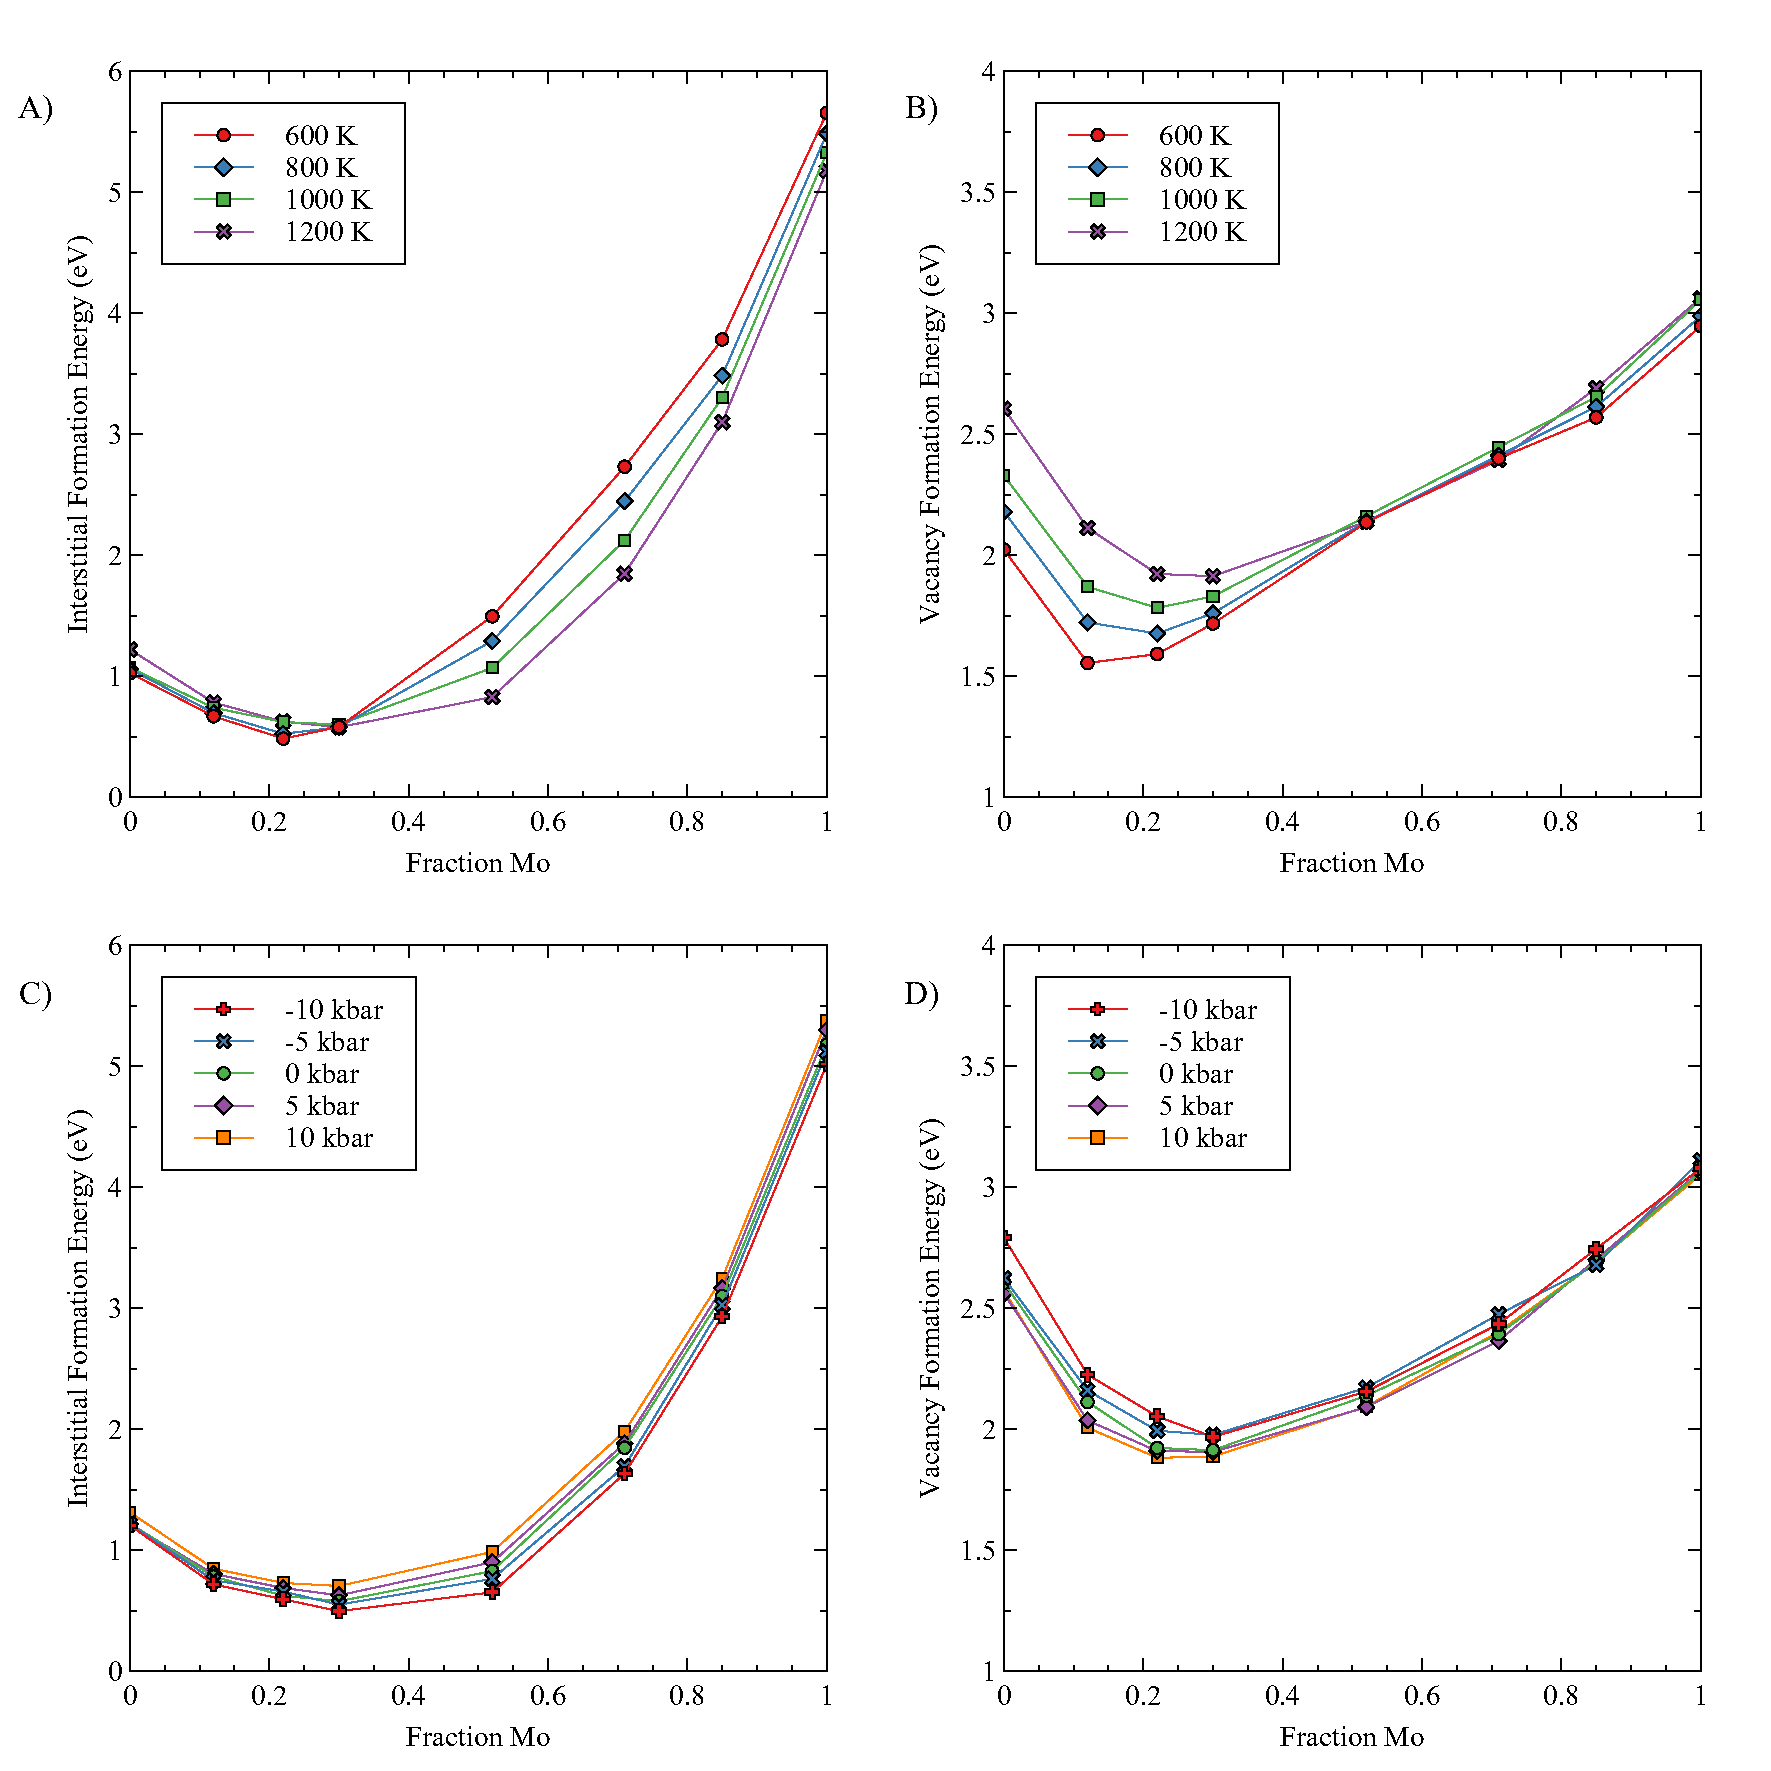
\includegraphics[width=0.9\textwidth]{figA.pdf}
\caption{The variation of point defect formation energies in U-Mo as a function of composition, temperature, and pressure. A) The interstitial formation energy as a function of composition at four temperatures. B) The vacancy formation energy as a function of composition at four temperatures. C) The interstitial formation energy as a function of composition at five pressures. D) The vacancy formation energy as a function of composition at five pressures.} 
\label{fig:A}
\end{figure}

The formation energy of interstitials and vacancies as a function of Mo atomic fraction at five unique pressures and a temperature of 1200 K is shown in Figures \ref{fig:A}C and \ref{fig:A}D. Vacancies and interstitials exhibit opposite trends as a function of applied pressure, as would be expected. As a crystal structure is compressed (positive pressure), atoms are closer together than in the equilibrium case. As such, it would be expected that a vacancy is more easily formed in the compressive state, and this is indeed observed. In the tensile state (negative pressure), atoms are farther apart than at equilibrium and there is additional space between the atoms. In this case, it would be expected that it is comparatively easier for an interstitial to form, and this is indeed observed. However, the pressure sensitivity is not uniform for defect type and composition, in that interstitials are the most sensitive to pressure at intermediate compositions (40-60 atomic percent), while vacancies are the most sensitive to pressure in the U-rich regime. 

The application of pressure does not affect the temperature dependence of defect formation energies, nor does the temperature affect the trends of applied pressure on defect formation energies. However, it does appear that at lower temperatures, the effects of pressure on interstitial formation energy are slightly dampened. If the pressure sensitivity is gauged as a matter of relative change of defect formation energies, it is found that generally, vacancies are much less sensitive to pressure than interstitials and that sensitivity is not significantly affected by the temperature. However, since the magnitude of the vacancy formation energy is larger than the magnitude of the interstitial formation energy, the absolute (not relative) change in the defect formation energy with applied pressure is approximately the same for both interstitials and vacancies. 

A note should be included on the choice of stress state. Only a hydrostatic stress state is applied in these systems. The actual stress state of the material may be more complex, consisting of bi-axial or uniaxial loading (shear loading is deemed unlikely). We have conducted preliminary studies on biaxial tension/compression and observed similar, but slightly lesser, trends in defect energetics. Prior studies have shown a dependence of defect behaviors on deformation volume change \cite{beeler2015,beeler2016}. Thus, it is expected that applied stress conditions that result in large volumetric changes (such as hydrostatic stress) will yield the largest defect response. Therefore, other stress states were not pursued further and the data presented in this manuscript can be considered an upper bound of the defect response to an applied stress.

The defect formation energies at all compositions, temperatures, and pressures are shown in \Cref{tab:EformI} and \Cref{tab:EformV}. 

\subsection{Formation Volumes and Dipole Tensors}

From \Cref{eq:enthalpy}, the formation volume of a point defect at a specified composition and temperature can be determined from the slope of the formation enthalpy with respect to pressure. The formation volume of interstitials and vacancies as a function of composition at different temperatures is shown in \Cref{fig:form_vol}.

\begin{figure}[h!]
    \centering
    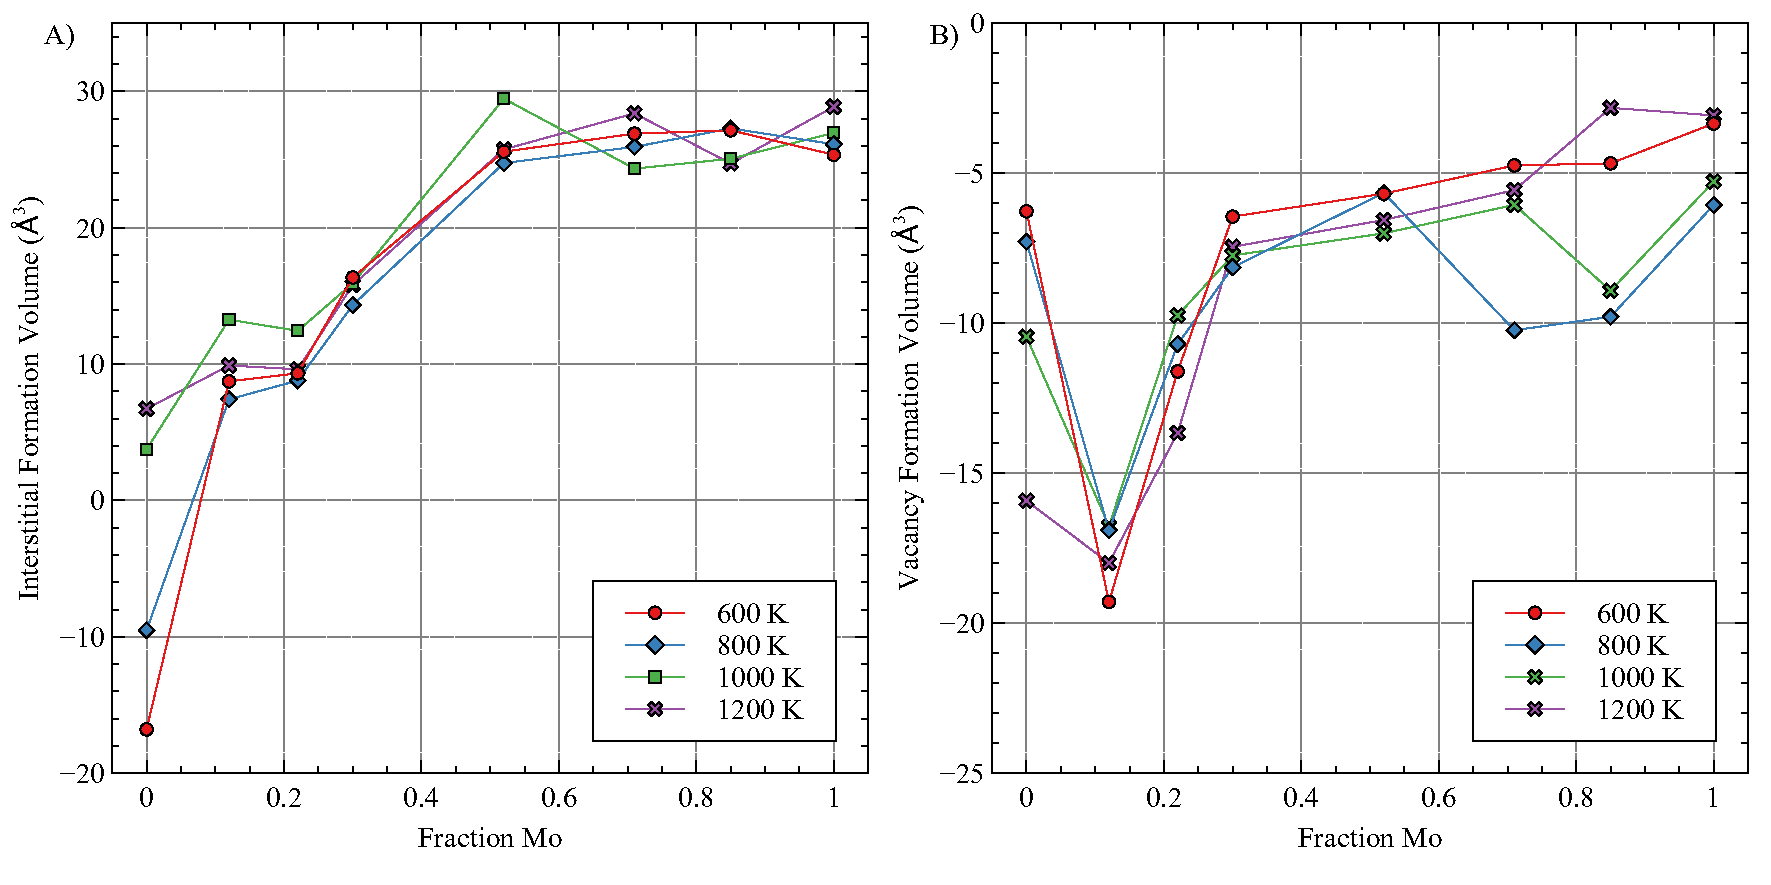
\includegraphics[width=0.8\textwidth]{form_vol.pdf}
    \caption{The defect formation volume of A) interstitials and B) vacancies in U-Mo alloys as a function of Mo content at four different temperatures.}
    \label{fig:form_vol}
\end{figure}

There are a number of interesting trends that emerge when analyzing the defect formation volumes. Let us begin by looking at the 1200 K data, where the interstitial shows a positive formation volume over the entire compositional range, and slightly increases with Mo content up to 50\% Mo, after which the defect formation volume is approximately constant. For vacancies, we observe negative formation volumes across the entire composition and again show a general increase with Mo content. The plateauing behavior for vacancies in U-Mo occurs for concentrations of greater than 30\% Mo. These are generally expected behaviors, but the compositional trends are novel to this system. For all alloy systems (non-zero concentration of Mo), these trends are generally consistent, showing some deviation, but retaining the same behaviors. There is some minor unexplained variance at high Mo content for the vacancy formation volume, however, the error bars (not shown for clarity) still overlap. For completeness, each data point shown in \Cref{fig:form_vol} is the product of a fit, and the standard error of that regression analysis was determined. These standard errors generally increase with temperature and decrease with higher Mo content. 

In exploring lower temperatures without Mo, we begin to deviate from the expected behavior. At 600 and 800 K, the interstitial has a negative defect formation volume. This indicates that with a higher compressive stress, the formation enthalpy of the interstitial decreases. As stated, this is counter-intuitive to our typical notion of the relationship between interstitials and pressure, in that they should have a lower formation enthalpy in systems under tension, where there is additional space in the lattice to accommodate them. There are two important points to note in order to properly contextualize this result. First is the difference between the relaxation volume and the formation volume. The relaxation volume is the change in the volume of a supercell upon the insertion of a defect. This relaxation volume is analogous to a change in pressure in a fixed-volume system, which is the case in this work, and will be discussed in the dipole tensor section. Thus, a negative formation volume does not equate to a negative relaxation volume. Second, the $\gamma$ phase of pure U is mechanically unstable at low temperatures \cite{beeler2010} and becomes stabilized with the addition of Mo. The interatomic potential utilized in this work can predict a metastable $\gamma$ phase at all temperatures investigated, however, based on the behavior of the formation volumes, it is clear that the U-rich structure is nearing the point of instability. Therefore, as we approach the stability limit of the $\gamma$ phase, an increase in the compressive stress leads to lower formation energies of interstitials. These stability effects are also observed for vacancies, in that as the temperature of pure $\gamma$ U decreases, the formation volume of vacancies increases (becomes less negative). This behavior is the converse of that observed for interstitials. It is our recommendation that defect formation volumes that indicate instability (those for $\gamma$ U below 1000 K), should not be utilized for higher-length scale studies. However, they are included here to demonstrate the behavior of this system, and how mechanical instabilities impact the thermodynamic behavior of defects, even if the structure itself remains stable. 

In the computation of the elastic dipole tensor using \Cref{eq:dipole2}, it was found that there are no significant off-diagonal components, and the induced stresses are isotropic (within the statistical certainty), which simplifies the calculation. Thus, the homogeneous stress is simply the trace of the stress tensor divided by 3. The elastic dipole tensor for U-Mo for interstitials and vacancies as a function of Mo content at four different temperatures is shown in \Cref{fig:dipole}.

\begin{figure}[h!]
    \centering
    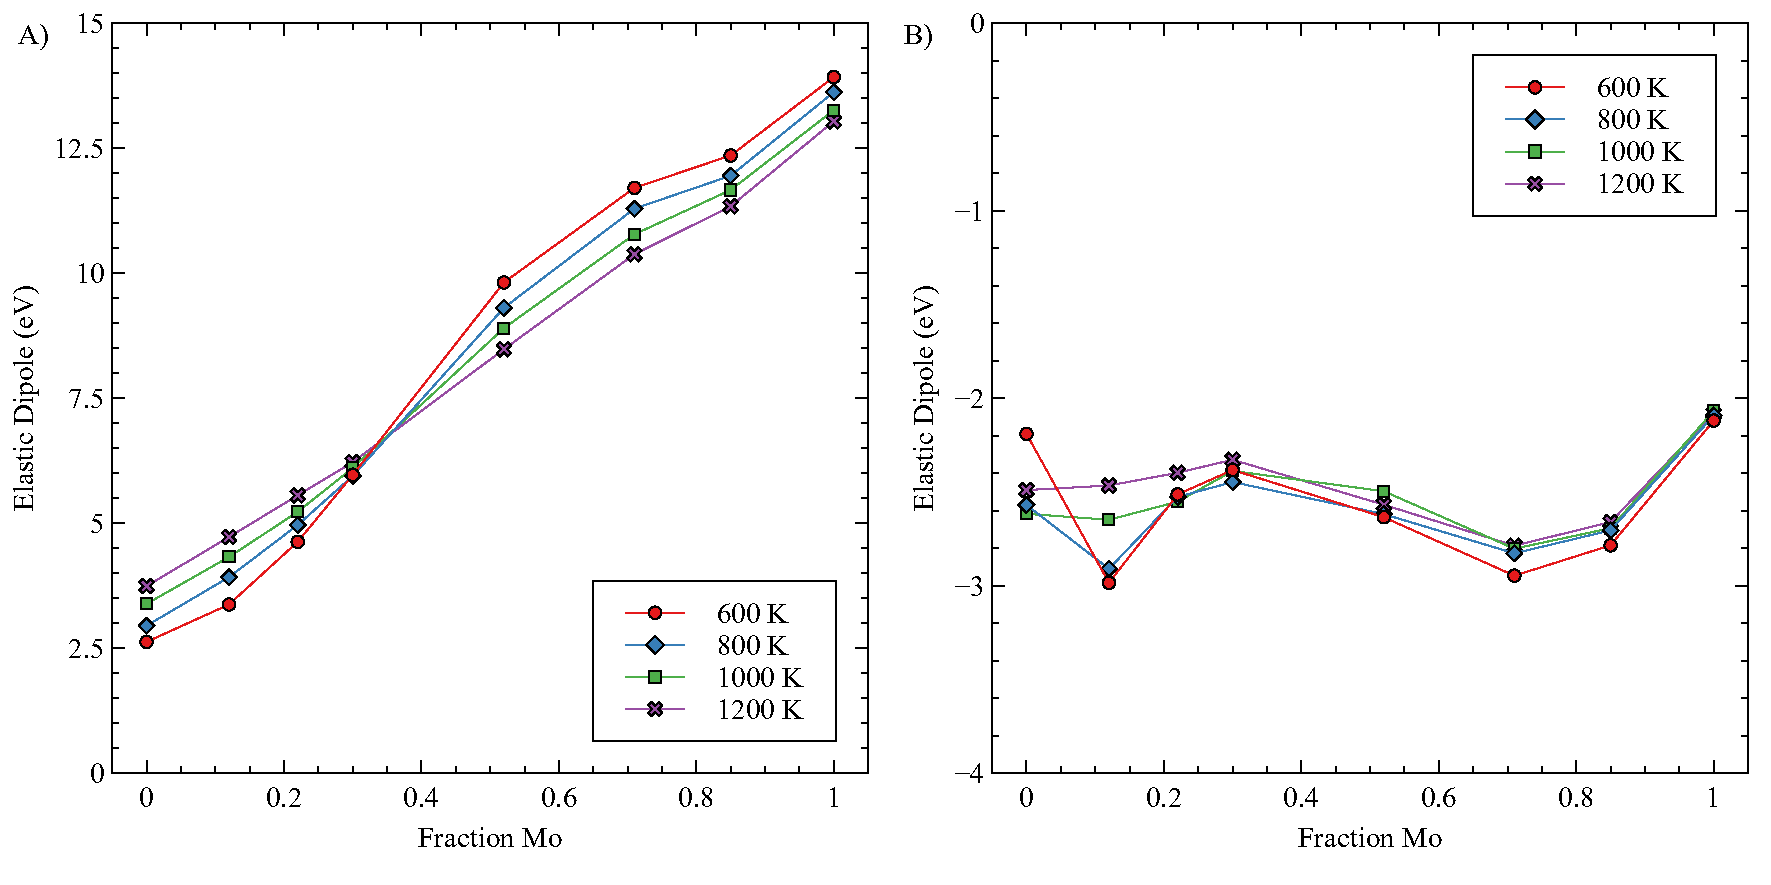
\includegraphics[width=0.8\textwidth]{dipole1.pdf}
    \caption{The elastic dipole tensor in U-Mo for A) interstitials and B) vacancies as a function of Mo content at four different temperatures.}
    \label{fig:dipole}
\end{figure}

The elastic dipole shows the relative amount of residual stress exerted by each species on the U-Mo system. Interstitials show clear trends with respect to both composition and temperature. The elastic dipole increases monotonically with increasing Mo content. However, there is an inflection point at 30\% Mo where the temperature trends reverse. Below this composition, an increase in temperature increases the elastic dipole, and above this composition, it decreases the elastic dipole. This inflection mirrors that of the formation energy shown in \Cref{fig:A}A. Thus, the formation energy is directly linked with the induced stress in the lattice from the inserted interstitial. The behavior of vacancies is more convoluted, as there are minimal changes across the entire compositional and temperature spectrum in the dipole tensor. The relative magnitude of the dipole tensor for vacancies is less than that of interstitials and possesses the opposite sign, indicating induced tensile stress instead of the observed compressive stress from interstitials. 

The impact of applied stress on the dipole tensor is also analyzed. For interstitials, there is a very slight positive correlation with pressure, in that a larger compressive stress leads to a higher elastic dipole. Vacancies have a similar magnitude trend, but in the opposite direction, exhibiting a lower elastic dipole under compressive stress. However, these effects are quite small, in that the total change in the elastic dipole for a given temperature and composition, considering the entire range of stresses (-10 to 10 kbar), is approximately 0.3 eV. This figure applies to both interstitials and vacancies, but, as stated, the direction of the impact is opposite for the two defect types. Thus, the magnitude of the stress has a minor impact on the defect elastic dipole. 

\subsection{Point Defect Diffusivities}

In this subsection, the diffusivities of interstitials and vacancies are studied as a function of composition, temperature, and pressure. This is the most thorough examination of point defect diffusive properties within the literature for zero pressure, and the only study to date exploring the effect of non-zero pressures. Data utilized to generate the plots in the following subsection are included in the appendix for completeness.

\subsubsection{Diffusion as a Function of Concentration}

The diffusion coefficient of interstitials and vacancies as a function of temperature for different U-Mo compositions is shown in \Cref{fig:diff_p0}. The plots for interstitials (A) and for vacancies (B) are shown on the same scale to make comparisons easier. Seven compositions are explored: bcc U, U-5Mo, U-10Mo, U-15Mo, U-30Mo, U-50Mo, and bcc Mo, where concentrations are given in weight percent. The temperature ranges over which diffusivities have been collected vary, as statistically significant diffusive behaviors are observed over different temperature regimes, due to the varying migration energies as a function of composition. 

The point defect diffusivity is always highest in bcc U, and tends to decrease with increasing Mo content. This decrease is monotonic for vacancies, in that bcc Mo displays the slowest diffusivity. However, for interstitials, the slowest diffusion is observed for U-50Mo. Typically, the slopes of these curves are less steep for interstitials than for vacancies, indicating smaller migration barriers, as expected. The migration barriers can be extracted from Arrhenius fits to each composition-defect data set. 

\begin{figure}[h!]
    \centering
    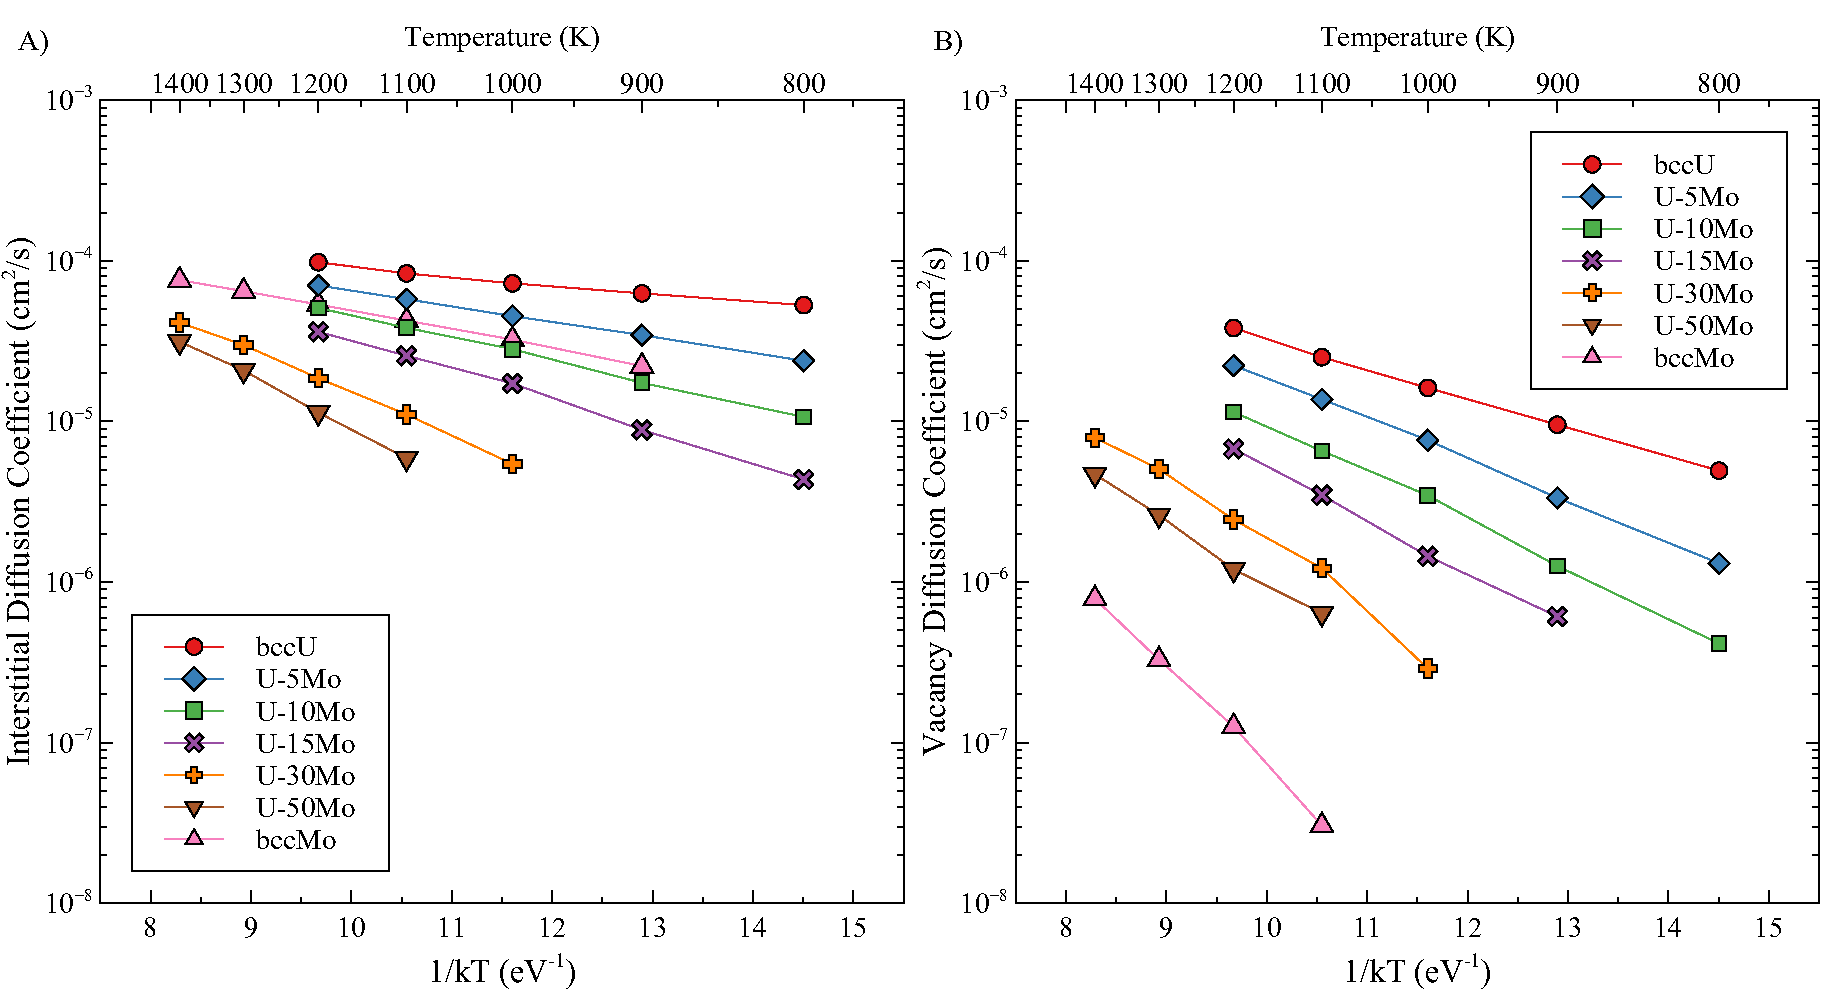
\includegraphics[width=0.9\textwidth]{diff_p0.pdf}
    \caption{The diffusion coefficient of A) interstitials and B) vacancies as a function of Mo concentration and temperature.}
    \label{fig:diff_p0}
\end{figure}

To more clearly illustrate the differences with respect to composition, the diffusion coefficient of interstitials and vacancies at 1200 K is plotted as a function of Mo concentration in \Cref{fig:1200K_diff}. There is a nearly linear function of the vacancy diffusion coefficient as a function of Mo, decreasing with additional Mo present within the alloy. However, for interstitials, there is a minimum at U-50Mo, and the diffusion coefficient increases for bcc Mo, to a level comparable to U-10Mo. To better elucidate the underlying effects, the migration barrier and the pre-factor for interstitials and vacancies as a function of Mo concentration are shown in \Cref{fig:Em_D0}. 

\begin{figure}[h]
    \centering
    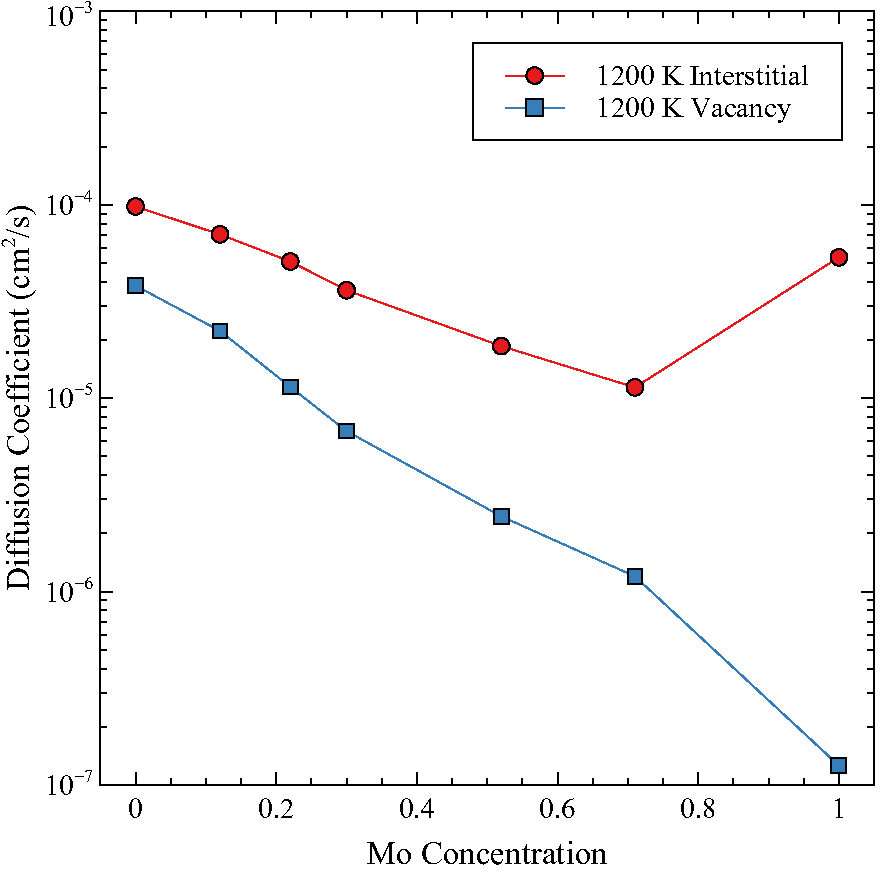
\includegraphics[width=0.5\textwidth]{1200K_diff.pdf}
    \caption{The diffusion coefficient of interstitials and vacancies as a function of Mo concentration at 1200 K.}
    \label{fig:1200K_diff}
\end{figure}

The migration barrier displays a very similar trend to the overall diffusivity, as would be expected, as this term lies within an exponential, and thus would likely have a stronger impact on the diffusivity than the prefactor. While monotonically decreasing for vacancies, the trend becomes less linear and is more appropriately fit by an exponential decay for concentrations from bcc U up to U-50Mo. This is followed by a steeper drop to the value of the migration energy for bcc Mo. It should be noted that migration barriers here are denoted as negatives, but this should be taken simply as the numerator in the Arrhenius function. This choice was made to more clearly illustrate comparisons between \Cref{fig:1200K_diff,fig:Em_D0}, in that a larger migration barrier (more negative value) decreases the diffusion coefficient. Thus, bcc Mo displays the highest migration barrier of all systems shown for vacancies. The interstitial migration barrier follows nearly an identical trend to the interstitial diffusivity shown in \Cref{fig:1200K_diff}. 

The prefactor shows more complex behavior but retains the discontinuity at a concentration of U-50Mo. The prefactor for interstitials displays an inverse behavior to that of the migration barrier, where it peaks at a concentration of U-50Mo and shows a minimum at bcc U. For vacancies, the prefactor is at a maximum for bcc Mo and a minimum for bcc U. In all of these systems, there is a clear delineation between the alloy behavior and the behavior of bcc Mo. Compositional dependence can readily be determined from bcc U up to U-50Mo, but there is a change in the diffusive behavior once Mo content exceeds 50 wt.\%. The origin of this piecewise-type behavior is unknown but potentially relates to the low-temperature instability of the bcc U phase and its potential impacts on modifying the alloy structure of U-Mo systems. Since higher Mo concentrations in the alloy were not studied (i.e., greater than 50 wt.\% but less than 100 wt.\%), the actual composition at which this inflection is present is unknown. Since U-rich Mo alloys are of primary interest, the Mo-rich portion of the alloy composition was sampled with less frequency in this work and is recommended as an area of potential future study. 

\begin{figure}[h!]
    \centering
    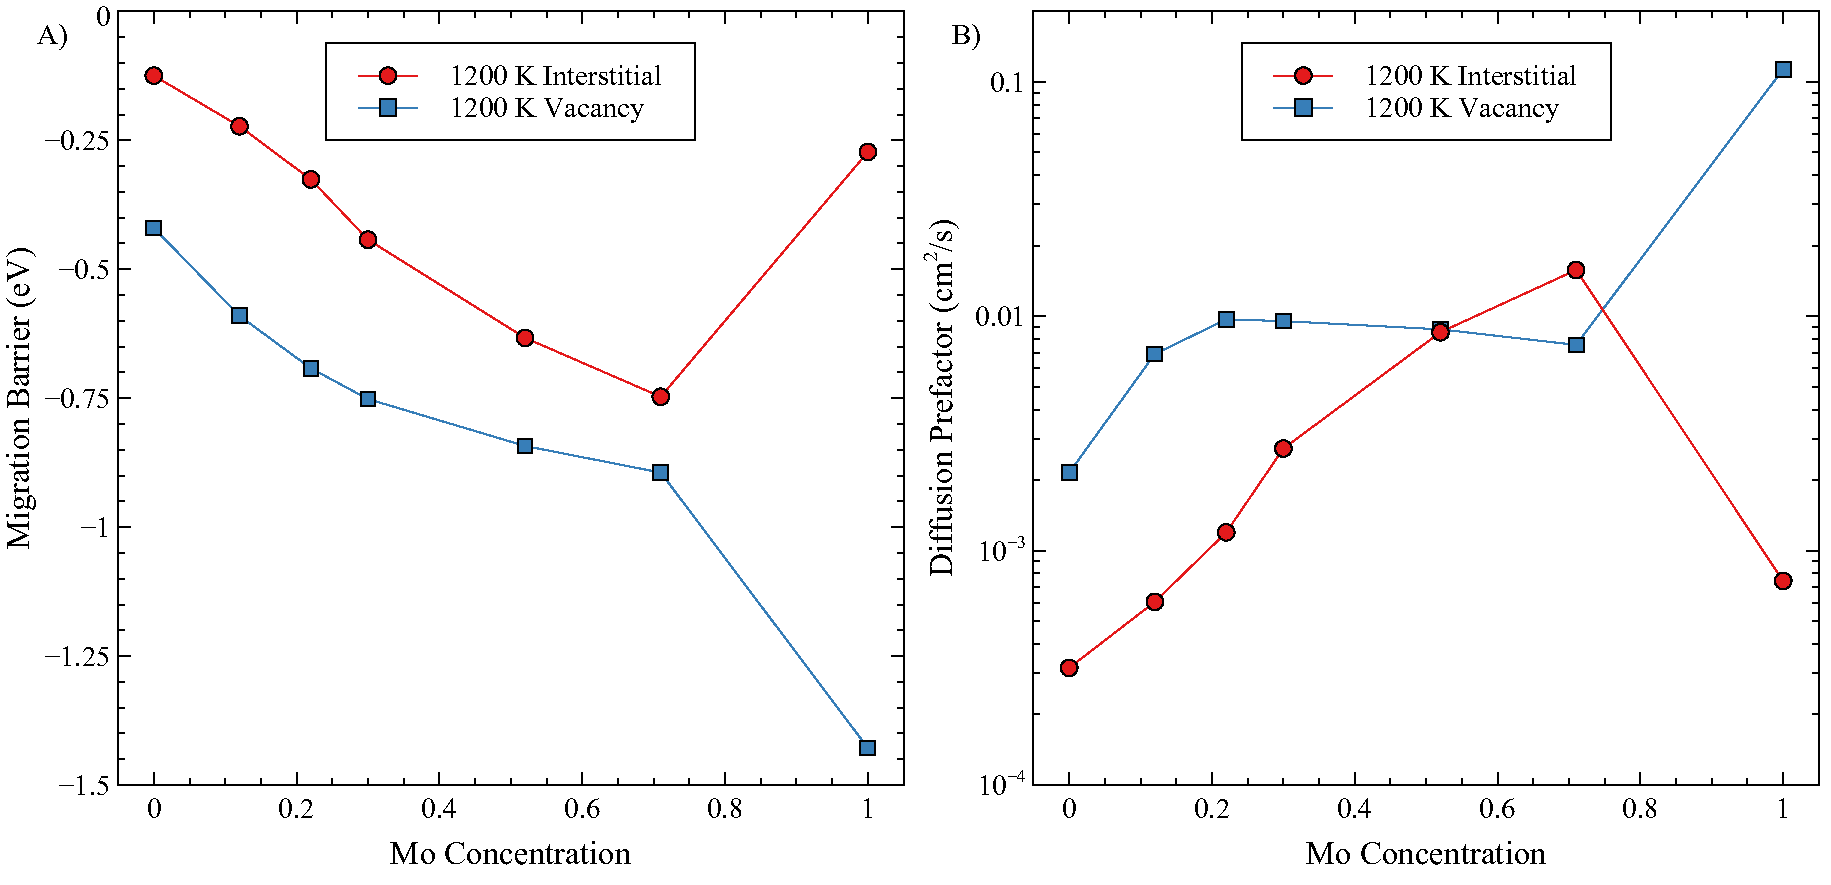
\includegraphics[width=0.9\textwidth]{Em_D0.pdf}
    \caption{The A) migration barrier and B) diffusion prefactor of interstitials and vacancies in U-Mo as a function of Mo concentration. The migration barrier shown is the numerator in the Arrhenius equation for ease of comparison.}
    \label{fig:Em_D0}
\end{figure}

\FloatBarrier

\subsubsection{Diffusion as a Function of Pressure}

The diffusion coefficient for interstitials and vacancies for U-10Mo as a function of applied pressure at five different temperatures is shown in \Cref{fig:int_vac_p}. As in the study on formation energies, hydrostatic pressure is applied, ranging from -10 to +10 kbar (-1 GPa to +1 GPa) in magnitude. The first observation is that the effects are quite minimal. For all data presented, the total magnitude of the diffusion coefficient changes by less than a factor of 2. Comparing this to the compositional effects presented earlier in this subsection where diffusion coefficients varied by up to 3 orders of magnitude, this indicates a nearly pressure-independent behavior. However, trends are present, albeit in a small magnitude. One would expect that for interstitials, a decrease in pressure, which yields an expansion of the lattice, would allow for faster interstitial diffusion. This is generally the case, where more negative pressures yield slightly higher diffusivities. For vacancies, we would expect the opposite trend, in that a compressive stress pushes atoms closer together, decreasing the jump path length, and subsequently increasing the vacancy diffusivity. This trend is not evident, as there is effectively no statistically significant difference in the vacancy diffusivity as a function of pressure. It should be noted that error bars are not shown on these plots for the sake of clarity, but all data shown has a standard deviation of less than 10\% for interstitials and less than 15\% for vacancies, with the standard deviation decreasing with increasing temperature. 

\begin{figure}[h!]
    \centering
    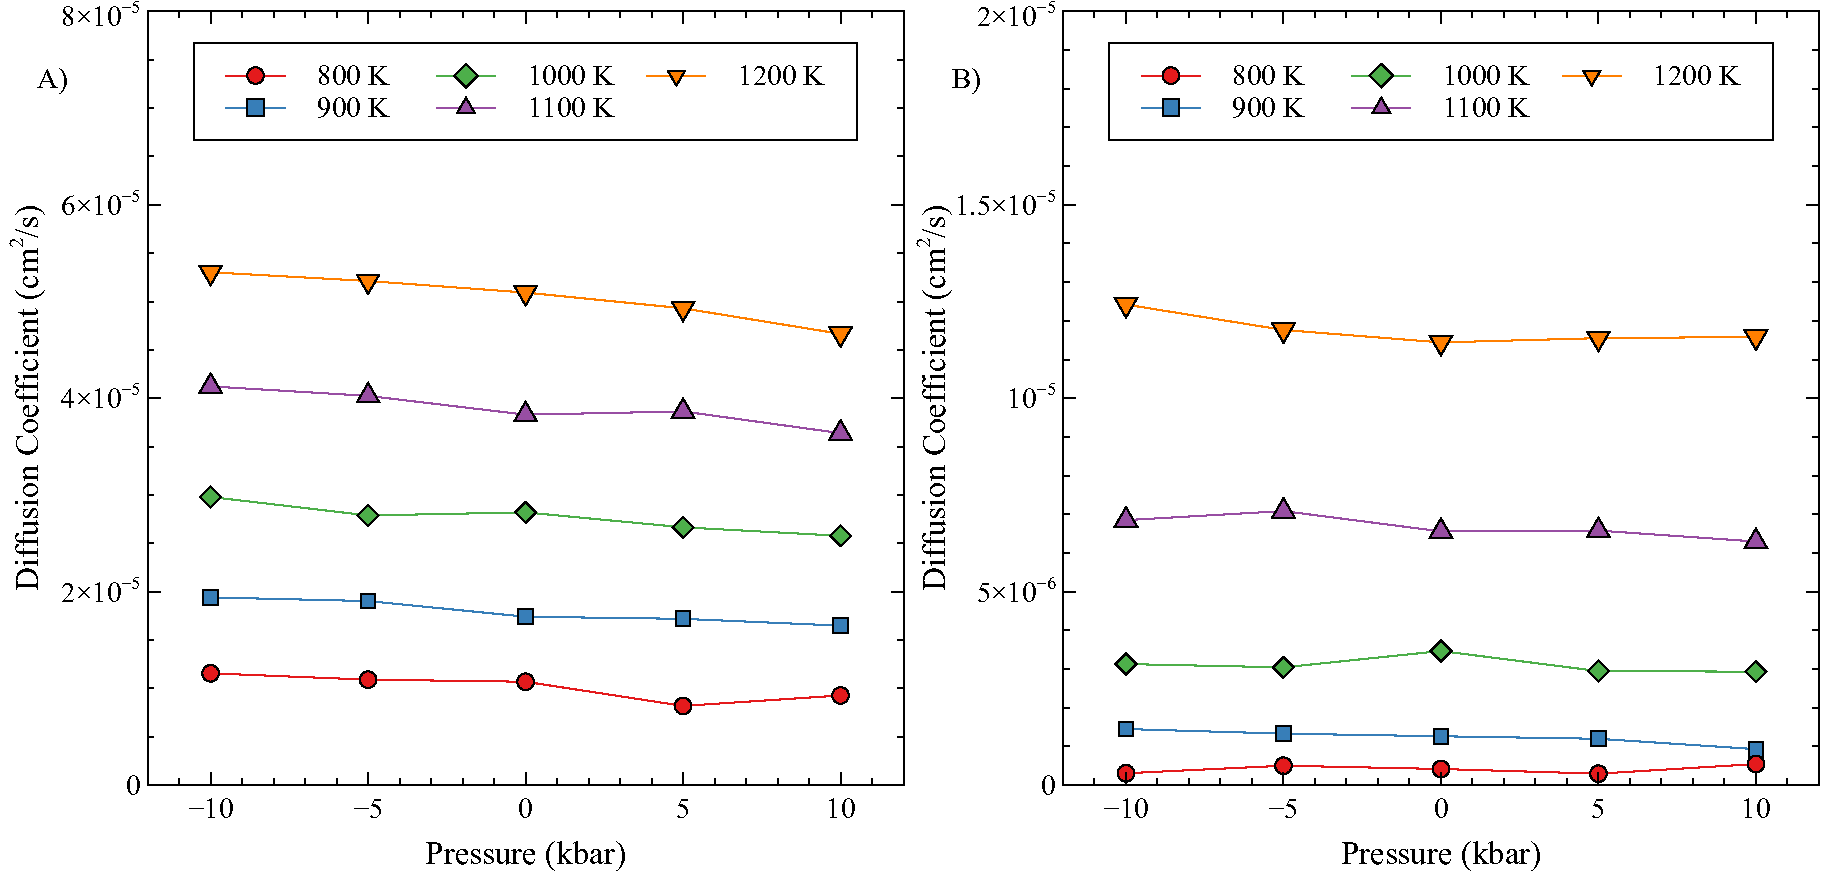
\includegraphics[width=0.9\textwidth]{int_vac_p.pdf}
    \caption{The diffusion coefficient of A) interstitials and B) vacancies in U-10Mo as a function of pressure.}
    \label{fig:int_vac_p}
\end{figure}

This data was analyzed as a function of temperature for all compositions and displayed a marginally greater influence of pressure at lower temperatures, but this finding was not statistically significant. Thus, the behaviors were averaged across temperatures to identify the general compositional trends with applied pressure. To do so, the slope of the diffusivity versus pressure data (displayed in \Cref{fig:int_vac_p}) was averaged over all temperatures explored at each composition. This slope versus pressure data tells us whether the diffusivity is positively (compressive stress increases diffusivity) or negatively (tensile stress increases diffusivity) correlated. This data is displayed in \Cref{fig:avg_vs_p}. For vacancies, the pressure has no statistically significant impact on diffusivity for Mo concentrations greater than U-5Mo. However, for bcc U, there is a pronounced impact in that compressive stresses increase vacancy diffusivity. For interstitials, there is a negative value of the slope of diffusivity versus pressure for all U-Mo compositions, indicating tensile stresses increase interstitial diffusivity. Interestingly, for bcc U, the interstitial diffusivity is slightly increased under compressive stresses. This may relate to a Crowdion mechanism \cite{crowdion} in bcc U which can potentially become more favorable under compressive stresses. However, this effect was not fully quantified. A slight positive correlation for interstitials in bcc Mo was also observed, but this result is not statistically significant, and thus it is concluded that applied pressure has a negligible impact on interstitial diffusivity in bcc Mo.

\begin{figure}[h!]
    \centering
    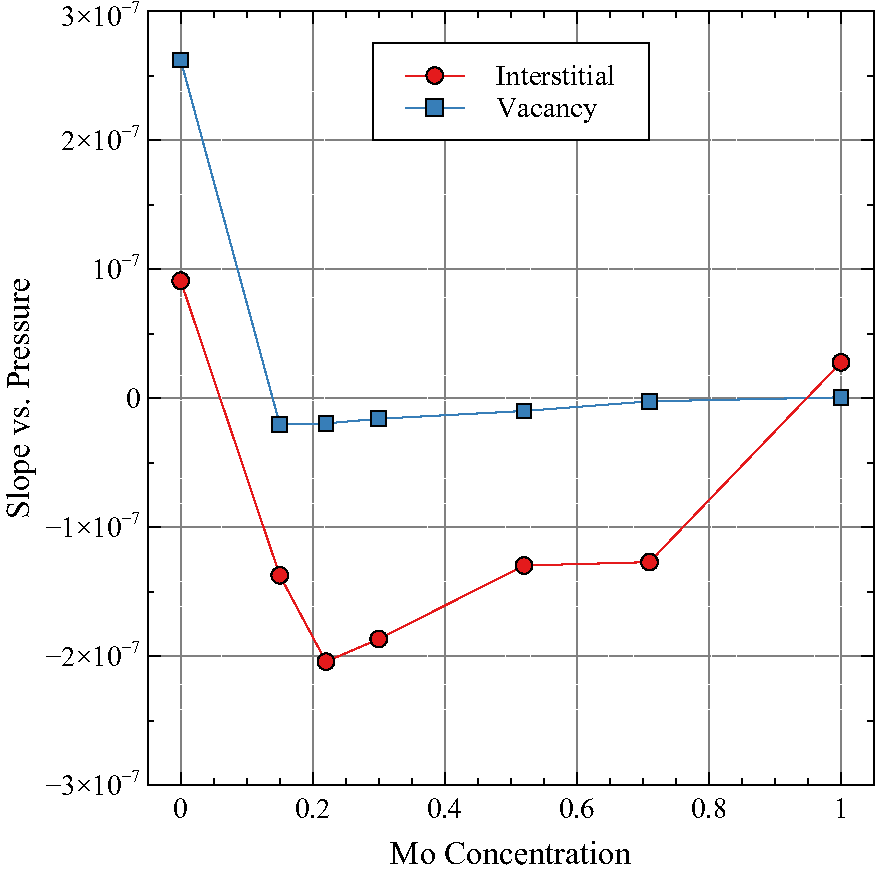
\includegraphics[width=0.6\textwidth]{avg_vs_p.pdf}
    \caption{The temperature-averaged slope of the diffusion coefficient versus pressure as a function of Mo concentration.}
    \label{fig:avg_vs_p}
\end{figure}

Thus, while there are clear trends identified for the effects of pressure on interstitial diffusivity, these impacts are quite small, and should only modify the magnitude of the defect diffusivity by less than a factor of two. Additionally, there is no statistically significant impact of pressure on vacancy diffusion for U-Mo alloys, but only for bcc U. To verify these findings in a more realistic scenario with variable stresses, diffusion under a pressure gradient was explored, as outlined in the following subsection. 

\FloatBarrier

\subsection{Diffusion Under a Pressure Gradient}

For the evaluation of point defect diffusion, a supercell with externally added force in one direction is simulated as described in the computational details. Figure \ref{fig:diff}A shows the resulting pressure gradient in the $x$-direction of the supercell. The simulation box is approximately 275 \r{A} long in the direction of the pressure gradient. The point defects, either an interstitial or a vacancy, are introduced at x = 137.5 \r{A}. The trajectories of the point defects are determined by tracking single lattice point jumps. Figure \ref{fig:diff}B depicts the point defect movement as colored vectors. A red vector denotes a jump by a U atom, while a blue vector denotes that of a Mo atom. The figure omits the $z$ coordinate for brevity. From the figure, it can be observed that the point defect movement is mainly facilitated by the U atoms with little help from the Mo atoms. There are two reasons for that: 1) U atoms make up 78 at.\% of the alloy, and 2) U atoms have a higher self-diffusivity than that of Mo atoms. Overall, the point defect motion resembles a random walk. To collect the statistics of point defect motion, data is aggregated from one thousand simulations for each type of point defect. Figure \ref{fig:diff}C displays violin plots with embedded boxplots of point defect final positions at the end of the simulations. The dashed vertical line in the middle represents the starting position of the point defects. The interquartile ranges of both types of point defects contain the initial position. The final positions of the vacancies are more centralized than that of interstitials. This is expected since interstitials generally move faster than vacancies. The mean final position of interstitials is $x = 125$ \r{A}, while the standard deviation is $40$ \r{A}. For vacancies, the mean is $x = 123$ \r{A}, and the standard deviation is $27$ \r{A}. Even though the mean final positions are toward the region with lower pressure for both types of point defects, we cannot conclude any directional preference due to the large standard deviations. As such, there is not enough evidence to claim that the pressure gradient in the alloy affects point defect diffusion.

\begin{figure*}[h!]
\centering
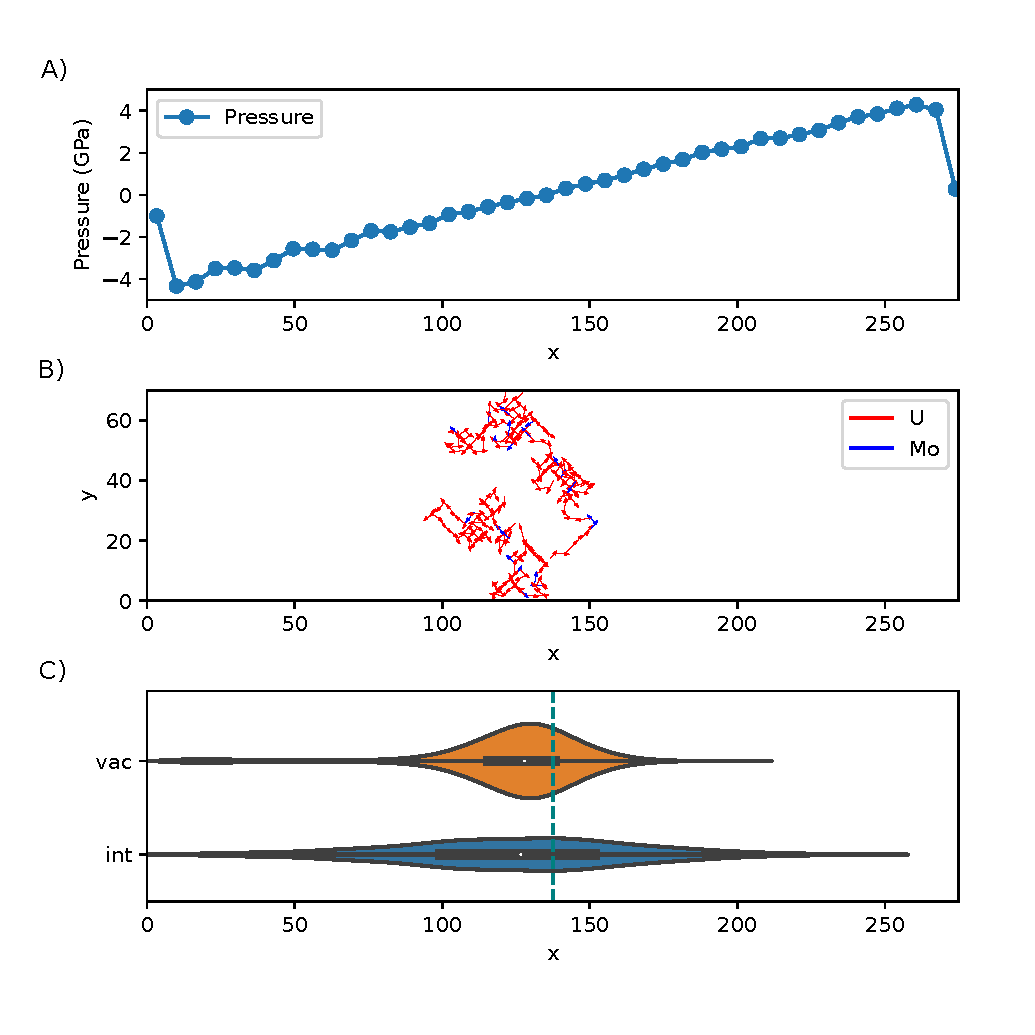
\includegraphics[width=0.9\textwidth]{PrGrad_2.pdf}
\caption{A) Pressure Gradient along the x-axis in the supercell. B) Trajectory of an interstitial defect. C) Violinplots with embedded boxplots of point defect (interstitials and vacancies) final positions at the end of simulations.}
\label{fig:diff}
\end{figure*}

\FloatBarrier

\subsection{Radiation Damage}

The number of defects generated in U-10Mo as a function of pressure for PKAs of 2, 4, 8, and 16 keV at 600, 800, 1000, and 1200 K is shown in \Cref{fig:rad_dam}. At lower temperatures, regardless of PKA energy, there is minimal effect of the pressure on the total number of defects generated. Every set of data displayed below 1200 K shows an effectively zero slope with respect to pressure. However, at 1200 K, there is a clear trend, in that compressive stresses (positive) inhibit the generation of defects, while tensile stresses (negative) enhance defect generation. The relative increase with applied pressure at 1200 K results in an increase in the number of defects generated of approximately 24\% for a -10 kbar tensile stress, and a corresponding decrease in the number of defects generated of approximately 14\% for a 10 kbar compressive stress. Error bars are not shown for the sake of clarity, but the standard deviation of the sample set is approximately 20\% of the mean value for each temperature, PKA energy, and pressure. 

\begin{figure}[h!]
    \centering
    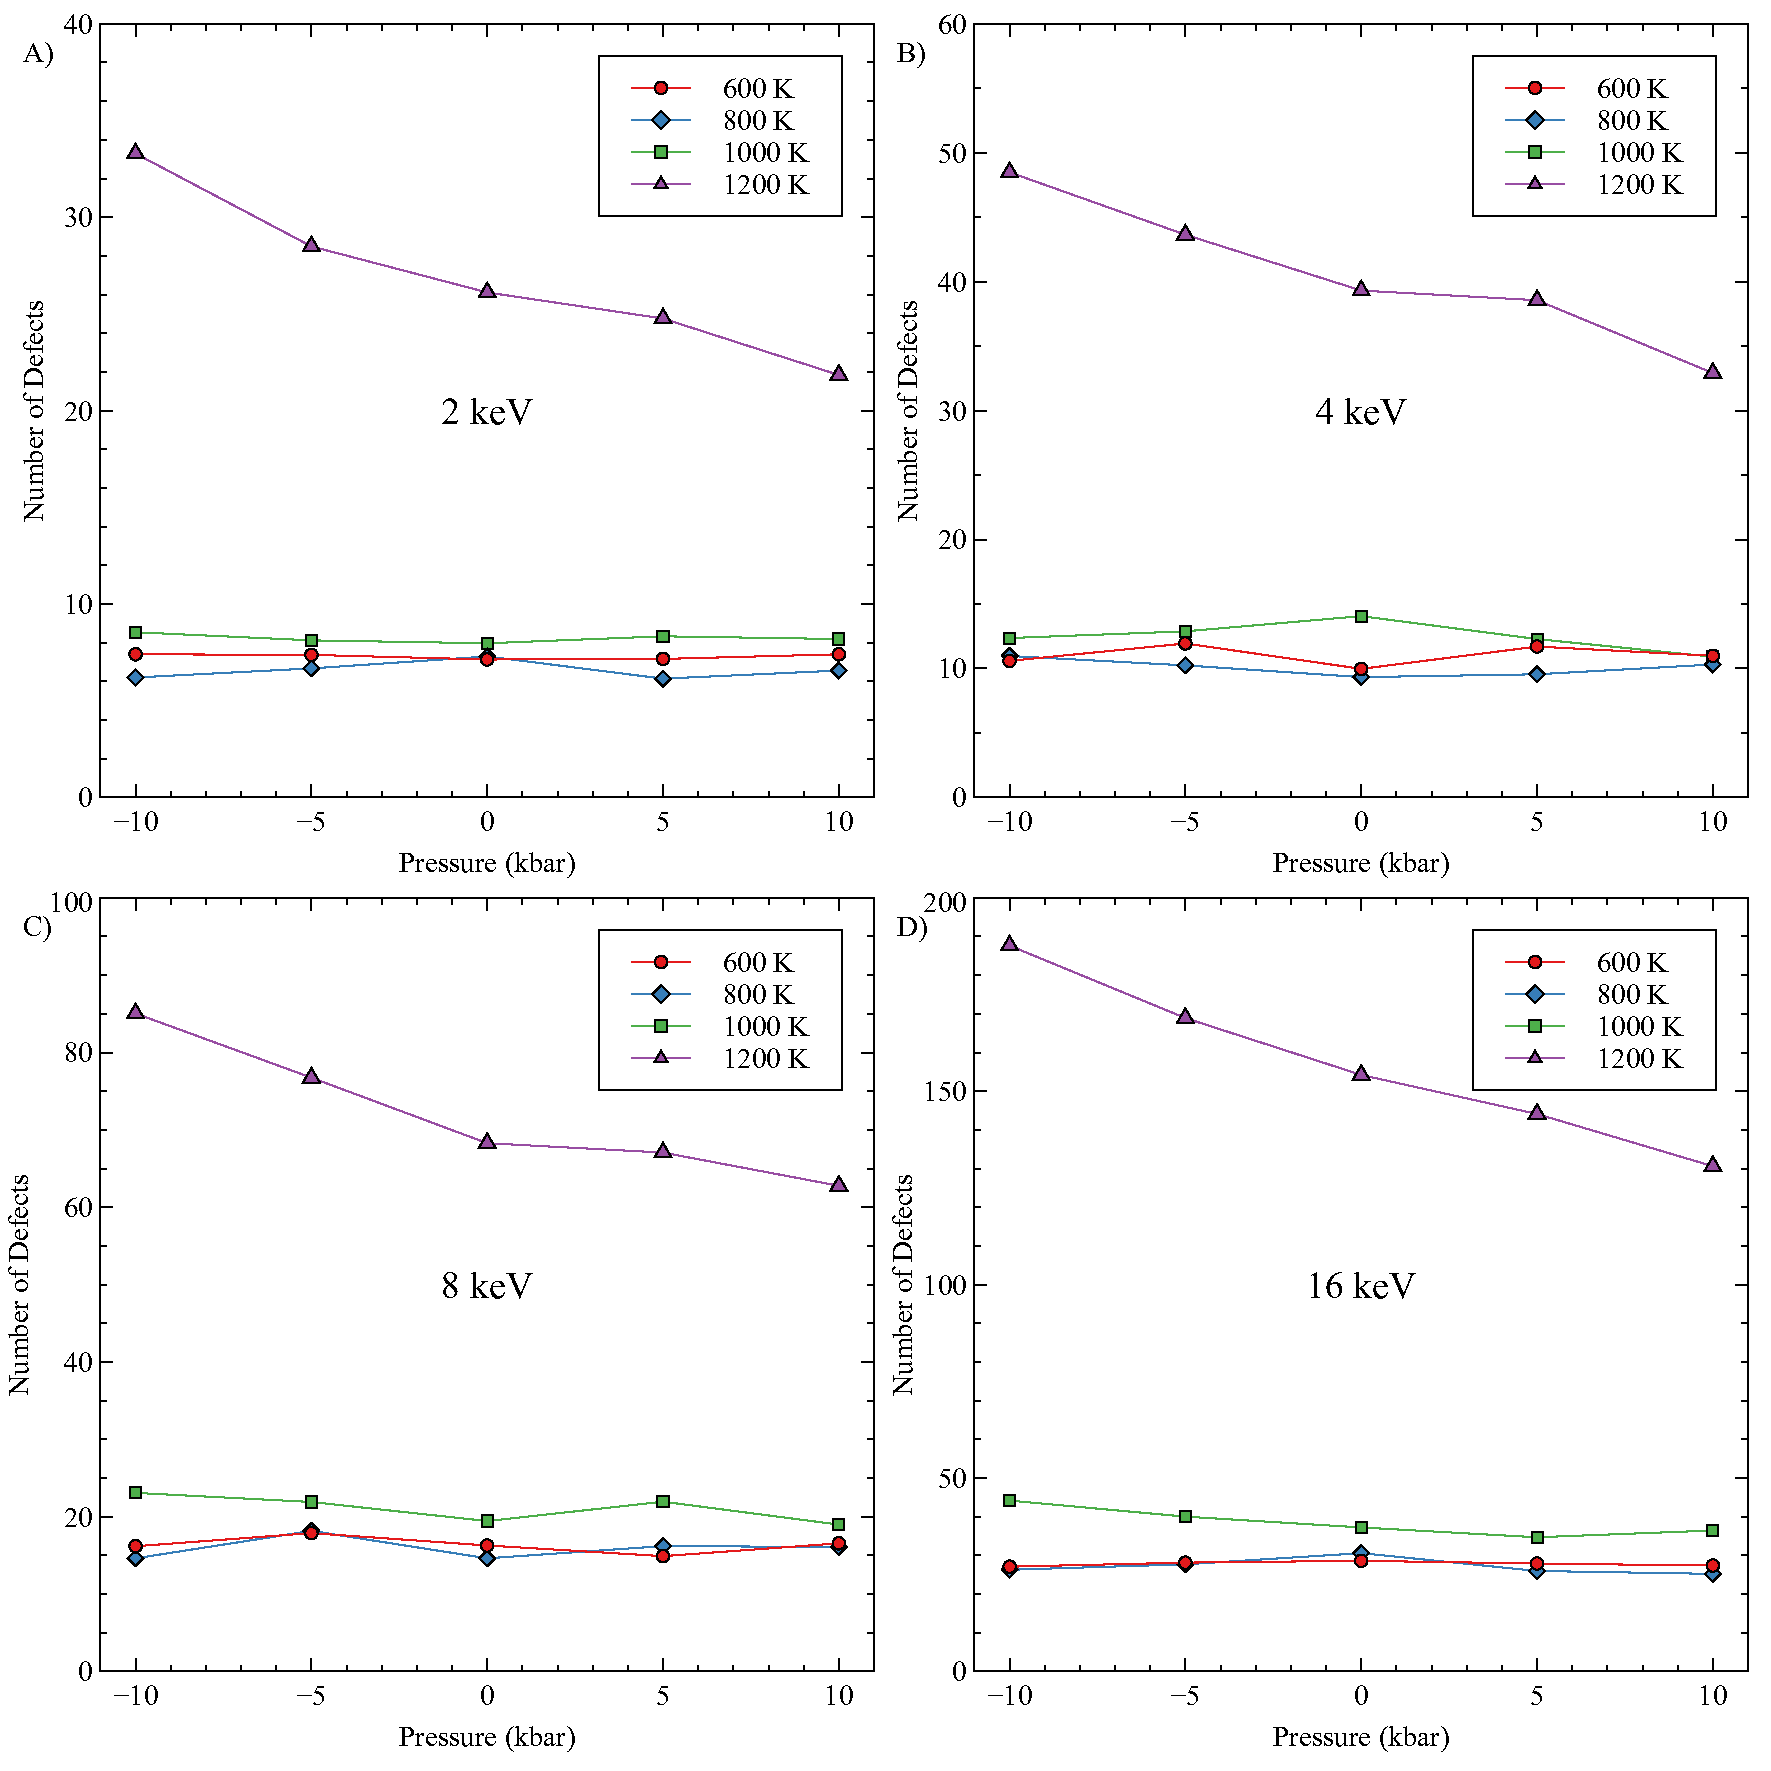
\includegraphics[width=0.9\textwidth]{rad_dam_P.pdf}
    \caption{The number of Frenkel pairs generated in U-10Mo as a function of pressure at four temperatures and PKA energies of (A) 2 keV, (B) 4 keV, (C) 8 keV, and (D) 16 keV.}
    \label{fig:rad_dam}
\end{figure}

The second trend observed from the figures is the increase in the number of defects with increasing temperature. From 600 to 800 K, there is no statistically significant difference in the number of defects. However, from 800 to 1200 K, the number of defects increases exponentially with the temperature for all PKA energies. The exponential increase takes the form of $ A \times e^{BT}$, where $A$ ranges from 0.33 to 0.68, and $B$ ranges from 0.0035 to 0.0044, with increasing values of $A$ and $B$ with increasing temperature. These trends are statistically significant, with $R^2 >$ 0.93. Thus, as the system approaches the melting point ($T>0.5T_m$), it becomes significantly easier to generate defects. This is despite the fact that for U-10Mo the defect formation energies slightly increase with increasing temperature. This is believed to be due to the fact that the cascade can more readily produce a localized melted zone during the thermal spike phase, producing more defects. For the primary application of interest in this work, research reactors, the operating temperature is below 600 K \cite{umo_prelim_report2017}. Thus, we do not expect to see significant effects of the pressure on defect generation, and we expect that the number of defects generated at temperatures below 600 K to be approximately equal to the data collected here at 600 K, due to the observed trends at higher temperatures. 

The collected data for each temperature at a zero pressure state are collected and displayed in \Cref{fig:def_power}. Power-law fits are obtained by examining the number of defects as a function of PKA energy at different temperatures. Power-law fits are chosen as they more readily fit MD data than the historical NRT \cite{norgett1975} or Kinchin-Pease (K-P) \cite{kinchin1955} equations, as in Miao \cite{miao2015}. The NRT/K-P models do not take into account recombination, as has been outlined by Nordlund \cite{nordlund2018}. The power-law fits change dramatically with increasing temperature, but converge at lower temperatures, with the data for 600 and 800 K essentially overlapping. All lower temperatures are expected to follow the behavior in these ``low temperature" curves. Such equations can be utilized to determine the number of residual defects from irradiation damage with more accuracy than the NRT model. 

\begin{figure}[h!]
    \centering
    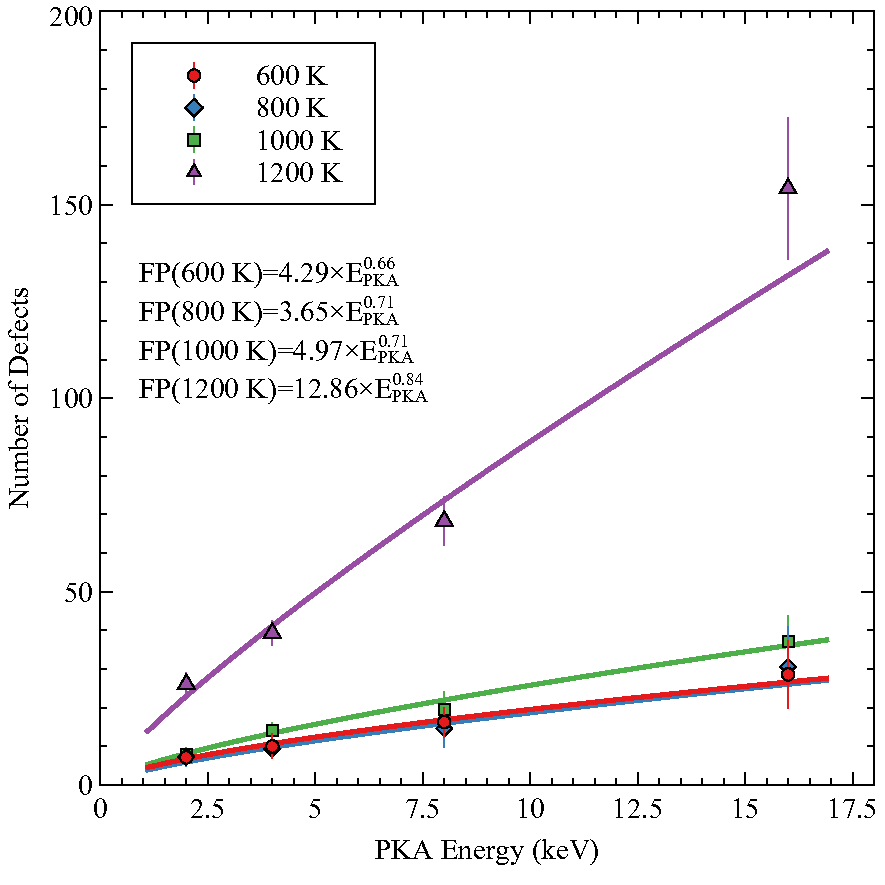
\includegraphics[width=0.6\textwidth]{FPvsE.pdf}
    \caption{The number of Frenkel pairs generated in U-10Mo as a function of PKA energy. Fits for each temperature of the form $A{\times}E_{PKA}^B$ are included, where $E_{PKA}$ is the PKA energy in keV.}
    \label{fig:def_power}
\end{figure}

It should be emphasized that radiation damage cascades were only conducted in U-10Mo, and thus there is no compositional dependence explored here. The fundamental nature of the residual radiation damage and the impact of composition are the subject of a future study. 

\FloatBarrier

\section{Conclusion}\label{sec4}
This work investigated how the hydrostatic tension and compression affect the formation energy of interstitials and vacancies as a function of pressure, temperature and composition in U-Mo. On average, the maximum applied pressure of 10 kbar produces a 6\% increase in the interstitial formation energy and a 3\% decrease in the vacancy formation energy. Under reasonable applied bulk pressures below the yield point ($<$100 MPa), negligible deviations in the defect formations are observed. There are impacts of the applied pressure on defect formation and clear trends can be observed, but these effects are sufficiently small, even at large pressures, that they likely can be neglected for practical purposes. However, in circumstances where the pressures may be quite large, e.g., in the area surrounding a highly pressurized nanometer-sized bubble, statistically significant changes in the local defect formation energy could be observed, potentially altering fission gas bubble evolution and creep behaviors. This work provides the basis for expansion to investigate the effects of applied pressure on defect diffusion, the behavior of defects under a stress gradient, and the generation of point defects due to applied pressure. 

\section{Acknowledgements}\label{sec5}
This work was supported by the U.S. Department of Energy, Office of Material Management and Minimization, National Nuclear Security Administration, under DOE-NE Idaho Operations Office Contract DE-AC07-05ID14517. This manuscript has been authored by Battelle Energy Alliance, LLC with the U.S. Department of Energy. The publisher, by accepting the article for publication, acknowledges that the U.S. Government retains a nonexclusive, paid-up, irrevocable, worldwide license to publish or reproduce the published form of this manuscript, or allow others to do so, for U.S. Government purposes. This research made use of the resources of the High Performance Computing Center at Idaho National Laboratory, which is supported by the Office of Nuclear Energy of the U.S. Department of Energy and the Nuclear Science User Facilities.

\section{Conflict of Interest}\label{sec6}
The authors declare no competing financial interest.

\section{Data Availability}\label{sec7}
Data will be made available upon request to the corresponding author. 

\section{Appendix}
\setcounter{figure}{0}
\setcounter{table}{0}
\renewcommand{\thefigure}{A\arabic{figure}}
\renewcommand{\thetable}{A\arabic{table}}

\subsection{Defect Formation Energies}

\begin{table}[h]
    \centering
     \caption{Formation Energy of Interstitials in U-Mo. Pressure in units of kbar and formation energies in units of eV.}
    \begin{tabular}{c|c|c|c|c|c|c|c|c}
    \toprule
 Pressure & bcc U & U-5Mo & U-10Mo & U-15Mo & U-30Mo & U-50Mo & U-70Mo & bcc Mo \\
 \hline
 \multicolumn{9}{c}{1200 K} \\
 \hline
 -10 & 1.21 &	0.72 &	0.60 &	0.50 &	0.65 &	1.64 &	2.93 &	5.01 \\
 -5 & 1.22 &	0.75 &	0.66 &	0.55 &	0.77 &	1.69 &	3.03 &	5.12 \\
 0 & 1.22 &	0.78 &	0.63 &	0.58 &	0.83 &	1.85 &	3.10 &	5.18 \\
 5 & 1.21 &	0.80 &	0.69 &	0.63 &	0.90 &	1.88 &	3.17 &	5.30 \\
 10 & 1.31 &	0.85 &	0.73 &	0.71 &	0.99 &	1.98 &	3.25 &	5.38 \\
 \hline
  \multicolumn{9}{c}{1000 K} \\
   \hline
-10	&1.05&	0.68&	0.53&	0.50&	0.84&	1.97&	3.13&	5.15 \\
-5	&1.08&	0.68&	0.57&	0.53&	1.00&	2.06&	3.23&	5.28 \\
0	&1.07&	0.74&	0.62&	0.60&	1.07&	2.12&	3.30&	5.33 \\
5	&1.10&	0.79&	0.66&	0.64&	1.13&	2.18&	3.34&	5.41 \\
10	&1.09&	0.83&	0.68&	0.69&	1.23&	2.29&	3.47&	5.51 \\
  \hline
  \multicolumn{9}{c}{800 K} \\
  \hline
-10	&1.12&	0.61&	0.50&	0.49&	1.10&	2.28&	3.33&	5.36 \\
-5	&1.09&	0.64&	0.52&	0.50&	1.19&	2.33&	3.41&	5.45 \\
0	&1.06&	0.70&	0.53&	0.58&	1.29&	2.45&	3.48&	5.48 \\
5	&1.04&	0.68&	0.56&	0.61&	1.37&	2.49&	3.59&	5.59 \\
10	&1.00&	0.70&	0.61&	0.66&	1.39&	2.60&	3.67&	5.70 \\
  \hline
  \multicolumn{9}{c}{600 K} \\
  \hline
-10	&1.14&	0.58&	0.43&	0.48&	1.33&	2.55&	3.60&	5.51 \\
-5	&1.09&	0.61&	0.44&	0.54&	1.42&	2.66&	3.69&	5.60 \\
0	&1.03&	0.67&	0.49&	0.58&	1.50&	2.73&	3.78&	5.66 \\ 
5	&0.96&	0.70&	0.51&	0.65&	1.56&	2.79&	3.86&	5.75 \\
10	&0.94&	0.68&	0.55&	0.68&	1.66&	2.91&	3.95&	5.83 \\
\hline
    \end{tabular}
    \label{tab:EformI}
\end{table}

\begin{table}[h]
    \centering
     \caption{Formation Energy of Vacancies in U-Mo. Pressure in units of kbar and formation energies in units of eV.}
    \begin{tabular}{c|c|c|c|c|c|c|c|c}
    \toprule
 Pressure & bcc U & U-5Mo & U-10Mo & U-15Mo & U-30Mo & U-50Mo & U-70Mo & bcc Mo \\
 \midrule
 \multicolumn{9}{c}{1200 K} \\
 \hline
-10	&2.79&	2.23&	2.05&	1.97&	2.16&	2.44&	2.75&	3.08 \\
-5	&2.62&	2.16&	1.99&	1.98&	2.17&	2.47&	2.68&	3.11 \\
0	&2.61&	2.11&	1.92&	1.91&	2.14&	2.39&	2.69&	3.06 \\
5	&2.56&	2.04&	1.91&	1.91&	2.09&	2.37&	2.70&	3.07 \\
10	&2.57&	2.01&	1.88&	1.89&	2.09&	2.40&	2.69&	3.05 \\
 \midrule
  \multicolumn{9}{c}{1000 K} \\
   \hline
-10	&2.40&	2.02&	1.86&	1.89&	2.18&	2.49&	2.71&	3.03 \\
-5	&2.37&	1.95&	1.84&	1.86&	2.18&	2.42&	2.70&	3.03 \\
0	&2.33&	1.87&	1.78&	1.83&	2.16&	2.45&	2.65&	3.06 \\
5	&2.26&	1.84&	1.77&	1.82&	2.13&	2.40&	2.64&	3.00 \\
10	&2.30&	1.82&	1.75&	1.79&	2.09&	2.40&	2.60&	2.96 \\
  \midrule
  \multicolumn{9}{c}{800 K} \\
  \hline
-10	&2.20&	1.85&	1.72&	1.81&	2.19&	2.49&	2.69&	2.99 \\
-5	&2.18&	1.73&	1.72&	1.80&	2.17&	2.45&	2.66&	3.00 \\
0	&2.18&	1.72&	1.68&	1.76&	2.14&	2.41&	2.61&	2.99 \\
5	&2.16&	1.67&	1.61&	1.72&	2.14&	2.38&	2.60&	2.95 \\
10	&2.09&	1.61&	1.61&	1.72&	2.12&	2.36&	2.57&	2.92 \\
  \midrule
  \multicolumn{9}{c}{600 K} \\
  \hline
-10	&2.03&	1.69&	1.67&	1.76&	2.18&	2.41&	2.61&	2.96 \\
-5	&2.01&	1.63&	1.61&	1.74&	2.16&	2.43&	2.60&	2.95 \\
0	&2.02&	1.56&	1.59&	1.72&	2.14&	2.40&	2.57&	2.95 \\
5	&1.99&	1.51&	1.56&	1.72&	2.14&	2.37&	2.56&	2.92 \\
10	&1.94&	1.46&	1.52&	1.67&	2.10&	2.36&	2.55&	2.92 \\
\bottomrule
    \end{tabular}
    \label{tab:EformV}
\end{table}

\FloatBarrier
\subsection{Defect Diffusion Coefficients}

\begin{table}[h]
    \centering
        \caption{Diffusion coefficients of interstitials fit to an Arrhenius function: $D=D_0 exp(-E_m/kT)$. $E_m$ is in units of eV and $D_0$ is in units of $cm^2/s$. }
    \label{tab:diff_int}
    \resizebox{\textwidth}{!}{%
    \begin{tabular}{c|cc|cc|cc|cc|cc}
    \toprule
         & \multicolumn{2}{c|}{-10 bar} & \multicolumn{2}{c|}{-5 bar} & \multicolumn{2}{c|}{0 bar} & \multicolumn{2}{c|}{5 bar} & \multicolumn{2}{c}{10 bar}   \\
    \midrule
        Composition & $E_m$ & $D_0$ & $E_m$ & $D_0$ & $E_m$ & $D_0$ & $E_m$ & $D_0$ & $E_m$ & $D_0$ \\
        \hline
        bcc U & 0.122 & 3.001 $\times 10^{-4}$ & 0.128 & 3.292 $\times 10^{-4}$& 0.125 & 3.160 $\times 10^{-4}$ & 0.122 & 3.094 $\times 10^{-4}$ &  0.121 & 3.075 $\times 10^{-4}$  \\
        U-5Mo & 0.221 & 6.087$\times 10^{-4}$ & 0.217 & 5.763$\times 10^{-4}$ & 0.223 & 6.048$\times 10^{-4}$ & 0.229 & 6.388$\times 10^{-4}$ & 0.233 & 6.576$\times 10^{-4}$ \\
        U-10Mo & 0.317 & 1.161$\times 10^{-3}$ & 0.323 & 1.204$\times 10^{-3}$ & 0.326 & 1.197$\times 10^{-3}$ & 0.370 & 1.884$\times 10^{-3}$ & 0.337 & 1.249$\times 10^{-3}$ \\
        U-15Mo & 0.434 & 2.792$\times 10^{-3}$ & 0.424 & 2.375$\times 10^{-3}$ & 0.443 & 2.727$\times 10^{-3}$ & 0.437 & 2.453$\times 10^{-3}$ & 0.483 & 3.908$\times 10^{-3}$ \\
        U-30Mo & 0.582 & 5.778$\times 10^{-3}$ & 0.575 & 5.044$\times 10^{-3}$ & 0.614 & 6.963$\times 10^{-3}$ & 0.593 & 5.537$\times 10^{-3}$ & 0.607 & 6.266$\times 10^{-3}$ \\
        U-50Mo & 0.758 & 1.824$\times 10^{-2}$ & 0.764 & 1.891$\times 10^{-2}$ & 0.747 & 1.576$\times 10^{-2}$ & 0.716 & 1.137$\times 10^{-2}$ & 0.773 & 1.786$\times 10^{-2}$ \\
        bcc Mo & 0.275 & 7.616$\times 10^{-4}$ & 0.272 & 7.352$\times 10^{-4}$ & 0.273 & 7.426$\times 10^{-4}$ & 0.266 & 7.025$\times 10^{-4}$ & 0.264 & 6.857$\times 10^{-4}$ \\
    \bottomrule
    \end{tabular}}
\end{table}

\begin{table}[h]
    \centering
        \caption{Diffusion coefficients of vacancies fit to an Arrhenius function: $D=D_0 exp(-E_m/kT)$. $E_m$ is in units of eV and $D_0$ is in units of $cm^2/s$. }
    \label{tab:diff_vac}
    \resizebox{\textwidth}{!}{%
    \begin{tabular}{c|cc|cc|cc|cc|cc}
    \toprule
         & \multicolumn{2}{c|}{-10 bar} & \multicolumn{2}{c|}{-5 bar} & \multicolumn{2}{c|}{0 bar} & \multicolumn{2}{c|}{5 bar} & \multicolumn{2}{c}{10 bar}   \\
    \midrule
        Composition & $E_m$ & $D_0$ & $E_m$ & $D_0$ & $E_m$ & $D_0$ & $E_m$ & $D_0$ & $E_m$ & $D_0$ \\
        \hline
        bcc U & 0.502 & 4.390$\times 10^{-3}$ & 0.461 & 3.129$\times 10^{-3}$ & 0.420 & 2.150$\times 10^{-3}$ & 0.401 & 1.880$\times 10^{-3}$ & 0.381 & 1.596$\times 10^{-3}$ \\
        U-5Mo & 0.598 & 7.794$\times 10^{-3}$ & 0.593 & 7.121$\times 10^{-3}$ & 0.590 & 6.906$\times 10^{-3}$ & 0.601 & 7.819$\times 10^{-3}$ & 0.607 & 8.209$\times 10^{-3}$ \\
        U-10Mo & 0.753 & 1.933$\times 10^{-2}$ & 0.663 & 7.189$\times 10^{-3}$ & 0.692 & 9.702$\times 10^{-3}$ & 0.758 & 1.891$\times 10^{-2}$ & 0.661 & 6.375$\times 10^{-3}$ \\
        U-15Mo & 0.803 & 1.675$\times 10^{-2}$ & 0.803 & 1.651$\times 10^{-2}$ & 0.752 & 9.540$\times 10^{-3}$ & 0.791 & 1.313$\times 10^{-2}$ & 0.821 & 1.831$\times 10^{-2}$ \\
        U-30Mo & 0.906 & 1.541$\times 10^{-2}$ & 0.797 & 5.700$\times 10^{-3}$ & 0.843 & 8.797$\times 10^{-3}$ & 0.824 & 6.677$\times 10^{-3}$ & 0.836 & 7.553$\times 10^{-3}$ \\
        U-50Mo & 0.904 & 8.768$\times 10^{-3}$ & 0.834 & 4.742$\times 10^{-3}$ & 0.894 & 7.550$\times 10^{-3}$ & 0.842 & 4.855$\times 10^{-3}$ & 0.894 & 8.043$\times 10^{-3}$ \\
        bcc Mo & 1.265 & 2.665$\times 10^{-2}$ & 1.228 & 1.960$\times 10^{-2}$ & 1.428 & 1.133$\times 10^{-1}$ & 1.211 & 1.711$\times 10^{-2}$ & 1.204 & 1.620$\times 10^{-2}$ \\
    \bottomrule
    \end{tabular}}
\end{table}


\FloatBarrier

\bibliographystyle{unsrt}
\bibliography{beelerbib}

\end{document}

